\documentclass[12pt, a4paper]{article}
\usepackage[utf8]{inputenc}
\usepackage[T1]{fontenc}
\usepackage{amsmath}
\usepackage{amssymb}
\usepackage{graphicx}
\usepackage{float}
\usepackage[hidelinks, breaklinks=true, hypertexnames=false]{hyperref}
\usepackage[top=1in, left=1in, right=1in, bottom=1.5in]{geometry}
\usepackage{lmodern}
\usepackage{fancyhdr}
\usepackage{xcolor}
\usepackage{booktabs}
\usepackage{multirow}
\usepackage{tabularx}
\usepackage{array}
\usepackage{enumitem}
\usepackage{listings}
\usepackage{tikz}
\usetikzlibrary{arrows.meta, positioning, shapes.geometric, fit, calc}

% --- Colours used in figures and code blocks ---
\definecolor{activepath}{rgb}{0.80,0.15,0.15}
\definecolor{idlenode}{rgb}{0.55,0.55,0.55}
\definecolor{stagefill}{rgb}{0.93,0.95,1.00}
\definecolor{codefill}{rgb}{0.97,0.97,0.97}
\definecolor{codecomment}{rgb}{0.35,0.45,0.35}

% --- Table helpers ---
\newcolumntype{L}{>{\raggedright\arraybackslash}X}
\newcolumntype{C}{>{\centering\arraybackslash}X}
\renewcommand{\arraystretch}{1.2}
\setlength{\tabcolsep}{5pt}
\setlength{\emergencystretch}{1.5em}
\setlength{\parindent}{0pt}

% Page breaks: \keepspace{<len>} before a heading starts a new page if less than
% <len> remains, and otherwise does nothing. Unlike \needspace it adds no bonus for
% breaking there, so LaTeX never jumps back to an earlier heading (leaving most of a
% page empty) when a later table or figure does not fit.
\makeatletter
\@secpenalty=0
\newcommand{\keepspace}[1]{\par\begingroup
  \setlength{\dimen@}{#1}%
  \dimen@ii\pagegoal \advance\dimen@ii-\pagetotal
  \ifdim\dimen@>\dimen@ii
    \ifdim\dimen@ii>\z@ \vfil\fi
    \break
  \fi\endgroup}
\makeatother

% --- Code blocks (netlists, commands) ---
\lstdefinestyle{block}{
    basicstyle=\ttfamily\footnotesize,
    backgroundcolor=\color{codefill},
    frame=single,
    rulecolor=\color{idlenode},
    breaklines=true,
    columns=fullflexible,
    keepspaces=true,
    showstringspaces=false,
    commentstyle=\color{codecomment},
    xleftmargin=0.5em,
    xrightmargin=0.5em,
    aboveskip=0.8em,
    belowskip=0.8em
}
\lstset{style=block}

% --- Header and Footer Configuration ---
\setlength{\headheight}{1.5cm}

\pagestyle{fancy}
\fancyhf{}

\fancyhead[L]{
\includegraphics[height=1cm]{IIITH_Logo.jpg}}
\fancyhead[R]{\nouppercase{\rightmark}}

\fancyfoot[L]{DVD Project: ML-Driven Leakage Estimation}
\fancyfoot[R]{\thepage}

\renewcommand{\headrulewidth}{0.4pt}
\renewcommand{\footrulewidth}{0.4pt}

% Every subsection re-issues its section's header mark, so a page that starts
% in the middle of one section and ends in the next is labelled with the
% section it starts in.
\newcommand{\currentsectionmark}{}
\renewcommand{\sectionmark}[1]{\gdef\currentsectionmark{\thesection\ #1}\markright{\currentsectionmark}}
\renewcommand{\subsectionmark}[1]{\markright{\currentsectionmark}}

\fancypagestyle{plain}{
    \fancyhf{}
    \fancyhead[L]{
\includegraphics[height=1cm]{IIITH_Logo.jpg}}
    \fancyhead[R]{\nouppercase{\rightmark}}
    \fancyfoot[L]{DVD Project: ML-Driven Leakage Estimation}
    \fancyfoot[R]{\thepage}
    \renewcommand{\headrulewidth}{0.4pt}
    \renewcommand{\footrulewidth}{0.4pt}
}

\fancypagestyle{tocpage}{
    \fancyhf{}
    \fancyfoot[L]{DVD Project: ML-Driven Leakage Estimation}
    \fancyfoot[R]{\thepage}
    \renewcommand{\headrulewidth}{0pt}
    \renewcommand{\footrulewidth}{0.4pt}
}

% --- Figures produced by the pipeline (report/ sits next to results/) ---
\graphicspath{{../results/}}

\begin{document}

% ==========================================
% TITLE PAGE
% ==========================================
\begin{titlepage}
    \centering
    
\includegraphics[width=0.6\linewidth]{IIITH_Logo.jpg}
    \vspace{1.5cm}

    {\fontfamily{cmr}\selectfont \Huge \textbf{DVD Course Project}}\\[0.3cm]
    {\fontfamily{cmr}\selectfont \LARGE Project Report}

    \vspace{1cm}

    \rule{0.9\linewidth}{1pt}
    \vspace*{0.5cm}

    \begin{minipage}{0.9\linewidth}
    \centering
    {\fontfamily{cmr}\selectfont \LARGE \textbf{ML-Driven PVT Variation Aware}} \\[0.3cm]
    {\fontfamily{cmr}\selectfont \LARGE \textbf{Leakage Estimation of CMOS Gates}} \\[0.3cm]
    {\fontfamily{cmr}\selectfont \LARGE \textbf{and a 3-bit Carry-Lookahead Adder}}
    \end{minipage}

    \vspace*{0.5cm}
    \rule{0.9\linewidth}{1pt}

    \vfill

    % ---------- Team name and four authors: two rows of two ----------
    {\fontfamily{cmr}\selectfont \Large \textbf{Team: The Current Affairs}}

    \vspace{0.8cm}

    \begin{minipage}[t]{0.45\linewidth}
        \raggedright
        \textbf{Author:} Vishnubhotla Nitin Sri Siva Kalyan \\
        \textbf{Roll:} 2024112012 \\
        \textbf{E-mail:} \\
        {\scriptsize \href{mailto:nitin.vishnubhotla@research.iiit.ac.in}{nitin.vishnubhotla@research.iiit.ac.in}}
    \end{minipage}%
    \hfill
    \begin{minipage}[t]{0.45\linewidth}
        \raggedright
        \textbf{Author:} Anay Rungta \\
        \textbf{Roll:} 2024102050 \\
        \textbf{E-mail:} \\
        {\scriptsize \href{mailto:anay.rungta@students.iiit.ac.in}{anay.rungta@students.iiit.ac.in}}
    \end{minipage}

    \vspace{0.8cm}

    \begin{minipage}[t]{0.45\linewidth}
        \raggedright
        \textbf{Author:} Alapati Sai Pavan Adit \\
        \textbf{Roll:} 2024102064 \\
        \textbf{E-mail:} \\
        {\scriptsize \href{mailto:saipavanadit.alapati@students.iiit.ac.in}{saipavanadit.alapati@students.iiit.ac.in}}
    \end{minipage}%
    \hfill
    \begin{minipage}[t]{0.45\linewidth}
        \raggedright
        \textbf{Author:} Vidvathama R \\
        \textbf{Roll:} 2024122002 \\
        \textbf{E-mail:} \\
        {\scriptsize \href{mailto:vidvathama.babu@research.iiit.ac.in}{vidvathama.babu@research.iiit.ac.in}}
    \end{minipage}

    \vspace{0.9cm}

    \textbf{GitHub Repo:} \href{https://github.com/NitinGamerX/DVD_Project}{https://github.com/NitinGamerX/DVD\_Project}

    \vfill

\end{titlepage}

\thispagestyle{tocpage}
\tableofcontents
\newpage

% ==========================================
% SECTION 1: SETUP
% ==========================================
\addtocontents{toc}{\protect\thispagestyle{tocpage}}
\section{Setup}
\label{sec:setup}

\noindent The project replaces SPICE leakage simulation with machine-learning (ML) models. Four models, one per transistor case (NMOS ON, NMOS OFF, PMOS ON, PMOS OFF), predict the four terminal currents of a single transistor under process, voltage and temperature (PVT) variation. From these models alone, the leakage of the INV, NAND2, NOR2, AND2 and OR2 gates and of the assigned test circuit is predicted and compared with SPICE. Table~\ref{tab:setup} lists the assigned configuration and the software used.

\begin{table}[H]
\centering
\small
\begin{tabularx}{\linewidth}{|>{\raggedright\arraybackslash}p{4.4cm}|L|}
\hline
\textbf{Item} & \textbf{Value} \\
\hline
Model file & PTM 22\,nm metal-gate / high-$k$ (\texttt{22nm\_MGK.pm}), BSIM4 level 54 \\
\hline
Nominal supply $V_{DD}$ & 1.0\,V \\
\hline
Test circuit & 3-bit carry-lookahead adder (CLA) with carry-in: 7 inputs, 128 input combinations \\
\hline
Simulator & ngspice 45.2 \\
\hline
Transistor geometry & $L = 22$\,nm, $W \in [1, 8] \times L_{\min}$; $AS = AD = W \cdot 44$\,nm, $PS = PD = 2(W + 44\,\text{nm})$ \\
\hline
ML software & Python 3.14.4, scikit-learn 1.9.1, NumPy 2.5.4, pandas 3.0.6 \\
\hline
\end{tabularx}
\caption{Assigned configuration and software.}
\label{tab:setup}
\end{table}

% ==========================================
% SECTION 2: DATA GENERATION
% ==========================================
\newpage
\addtocontents{toc}{\protect\thispagestyle{tocpage}}
\section{Data Generation}
\label{sec:data}

\keepspace{251pt}
\subsection{Sampling}
\noindent For each case, every sample draws all inputs independently from the distributions in Table~\ref{tab:sampling}, with $V_{DD}$ drawn first because the ranges of $V_d$ and $V_s$ depend on it. The gate and body voltages are fixed by the case: $V_g = V_{DD}$ for NMOS ON and PMOS OFF and 0 otherwise; $V_b = 0$ for NMOS and $V_{DD}$ for PMOS. Each case uses its own fixed random seed.

\begin{table}[H]
\centering
\small
\begin{tabularx}{\linewidth}{|>{\raggedright\arraybackslash}p{4.6cm}|L|}
\hline
\textbf{Input} & \textbf{Distribution} \\
\hline
$V_{DD}$ & Uniform, $1.0\,\text{V} \pm 10\,\%$ \\
\hline
$V_d$, $V_s$ & Uniform, $[0, V_{DD}]$, independently \\
\hline
Width $W$ & Uniform, $[1, 8] \times L_{\min}$ \\
\hline
Temperature & Uniform, $[-40, 125]\,^{\circ}$C \\
\hline
\texttt{vth0}, \texttt{toxe}, \texttt{ndep}, \texttt{u0}, \texttt{xj} & Uniform, nominal value of the model file $\pm 10\,\%$ \\
\hline
\end{tabularx}
\caption{Sampling distributions.}
\label{tab:sampling}
\end{table}

\keepspace{220pt}
\subsection{Netlists}
\noindent Each sample is simulated with a single-transistor netlist in which every terminal has its own voltage source and the source and drain areas and perimeters are specified. The five process parameters enter as SPICE parameters of a copy of the model file in which only they are parametrized. The structure is:

\noindent\begin{minipage}{\linewidth}
\begin{lstlisting}
.include 22nm_MGK_param.pm   * model file; vth0, toxe, ndep, u0, xj as .param
.options gmin=1e-18 abstol=1e-18 reltol=1e-6 vntol=1e-9
.temp {T}
M1 d g s b nmos W={W} L=22n AS={W*44n} AD={W*44n} PS={2*(W+44n)} PD={2*(W+44n)}
Vd d 0 {Vd}
Vg g 0 {Vg}
Vs s 0 {Vs}
Vb b 0 {Vb}
.op
\end{lstlisting}
\end{minipage}

\noindent The recorded currents are the source branch currents $I(V_d)$, $I(V_g)$, $I(V_s)$, $I(V_b)$. Gate and test-circuit netlists use the same model card, options line and diffusion geometry, with one source per primary input.

\keepspace{14\baselineskip}
\subsection{Data Split}
\noindent Each of the four datasets has 10,000 rows and is split randomly with a fixed seed into training (70\,\%, 7,000 rows), validation (15\,\%, 1,500) and test (15\,\%, 1,500) sets. The validation set is used only for model selection and the test set only for the final evaluation of the chosen models.

\medskip
\noindent Inside a gate, every transistor terminal sits within a few millivolts of a rail, a region that uniform sampling of $V_d$ and $V_s$ rarely visits (0.4\,\% of terminals lie within 2\,mV of a rail). The improved models (Section~\ref{sec:improved}) therefore also use additional training data: 20,000 further uniform samples per case, and 10,000 \emph{rail-focused} samples per case in which $V_d$ and $V_s$ are each, with probability 0.5, placed a log-uniform distance of 1\,$\mu$V to 0.3\,V from a rail. The rail-focused samples are split 70/15/15 in the same way, giving a separate rail validation and test set.

\keepspace{205pt}
\subsection{Data Check}
\noindent For every sample the four terminal currents must sum to zero within the solver tolerance, $|\Sigma I| \le 10^{-6}\,\Sigma|I| + 10^{-13}$\,A. All 40,000 samples pass (Table~\ref{tab:kcl}); the residuals are double-precision rounding noise.

\begin{table}[H]
\centering
\small
\begin{tabularx}{\linewidth}{|L|c|c|c|}
\hline
\textbf{Case} & \textbf{Passed} & \textbf{Median $|\Sigma I|$ (A)} & \textbf{Max $|\Sigma I|$ (A)} \\
\hline
NMOS ON & 10,000 / 10,000 & $8.8\times10^{-17}$ & $1.8\times10^{-15}$ \\
\hline
NMOS OFF & 10,000 / 10,000 & $4.4\times10^{-24}$ & $5.6\times10^{-22}$ \\
\hline
PMOS ON & 10,000 / 10,000 & $8.7\times10^{-18}$ & $1.1\times10^{-16}$ \\
\hline
PMOS OFF & 10,000 / 10,000 & $3.9\times10^{-16}$ & $1.2\times10^{-14}$ \\
\hline
\end{tabularx}
\caption{Kirchhoff check of the four datasets.}
\label{tab:kcl}
\end{table}

\noindent Figures~\ref{fig:trend_t}--\ref{fig:trend_tox} show the three required trends, each overlaid with a controlled SPICE sweep of the single parameter. All three have the expected direction. The OFF current rises with temperature ($\times$15 for NMOS and $\times$9 for PMOS from $-40$ to $125\,^{\circ}$C), less steeply than its sub-threshold channel part ($\times$64 and $\times$15) because the temperature-independent gate tunnelling current carries 78\,\% (NMOS) and 42\,\% (PMOS) of it at $-40\,^{\circ}$C. The channel part falls by one decade per 81--82\,mV of threshold voltage, and the gate current falls by about 0.8 decades per \AA{} of oxide thickness in all four cases.

\begin{figure}[H]
\centering
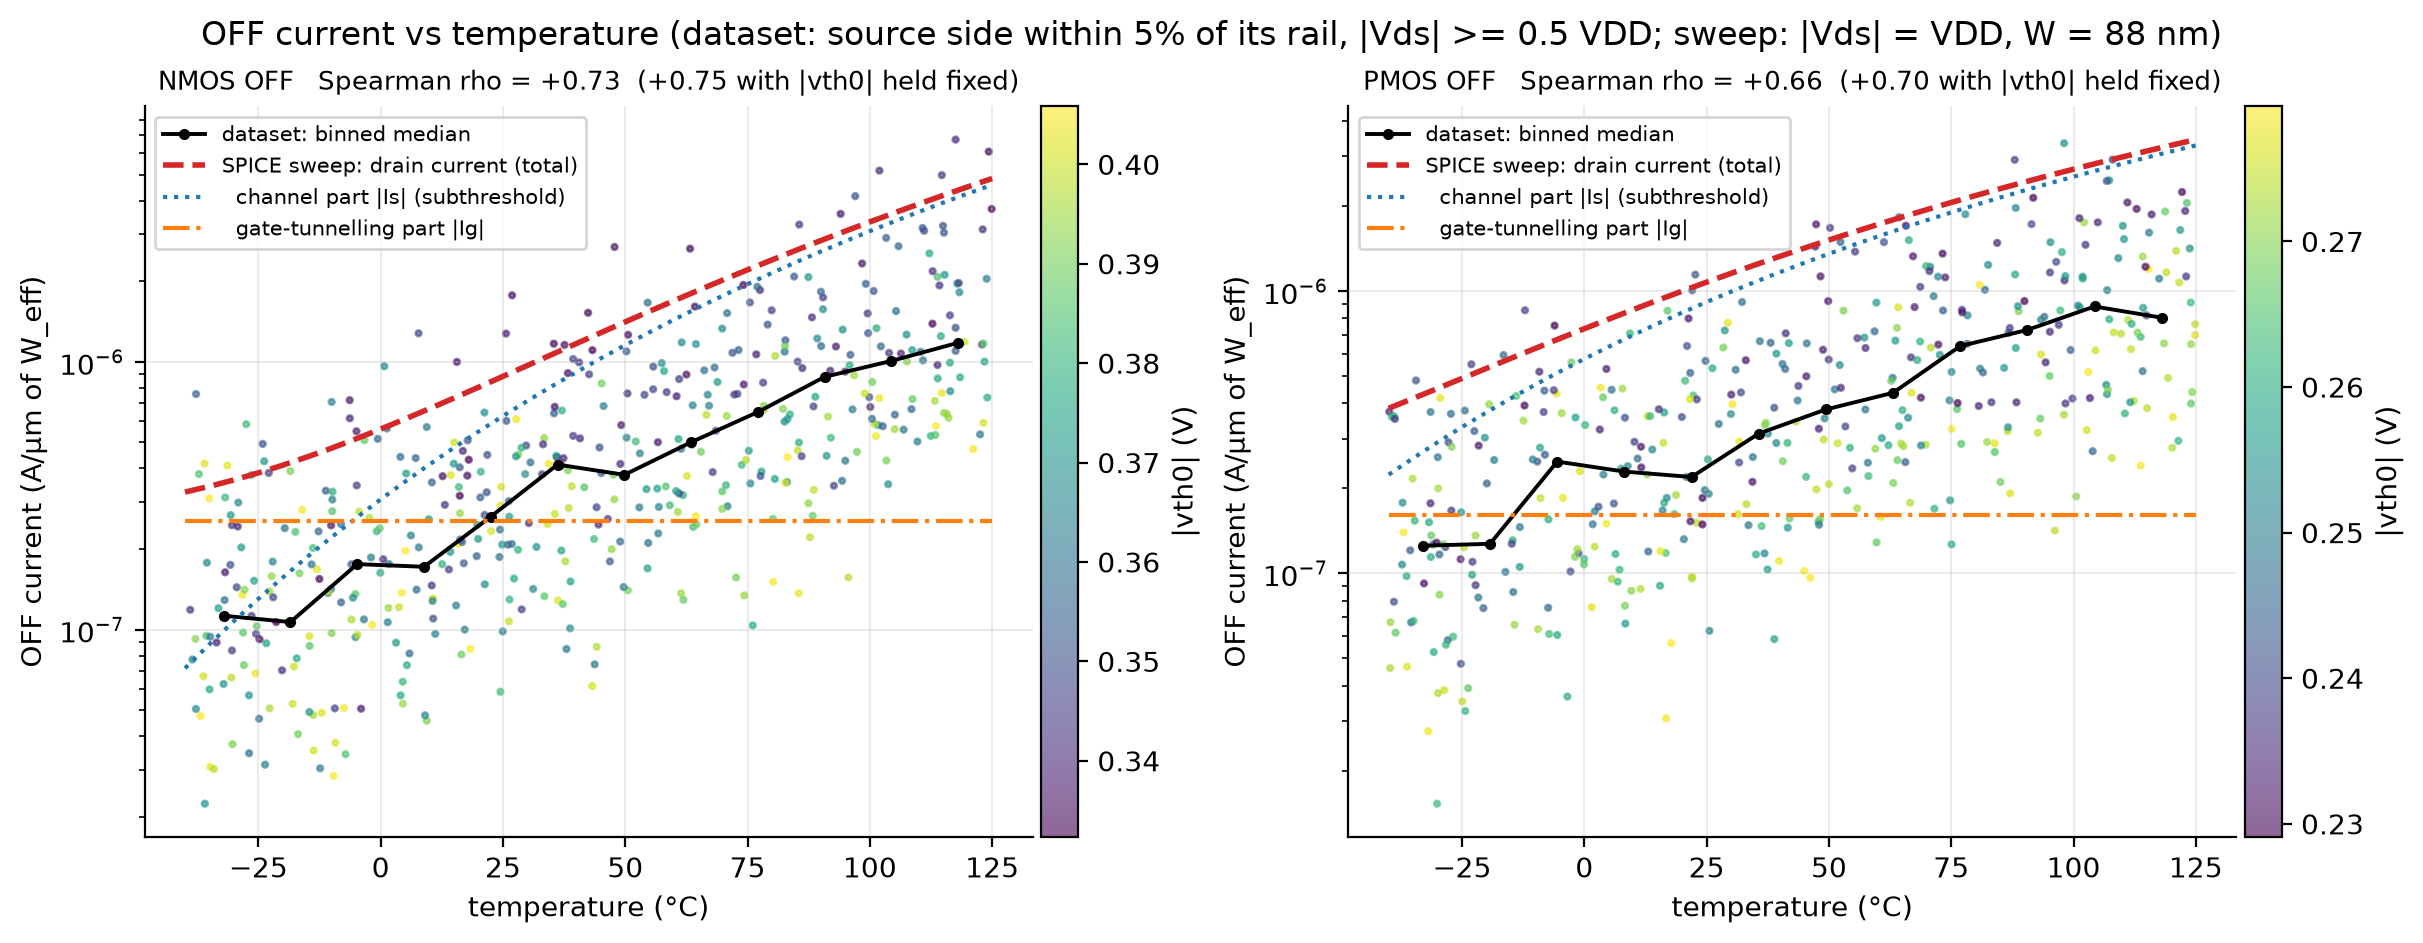
\includegraphics[width=\linewidth]{data_check/off_current_vs_temperature.png}
\caption{OFF current versus temperature, with the sweep split into its channel and gate-tunnelling parts.}
\label{fig:trend_t}
\end{figure}

\begin{figure}[H]
\centering
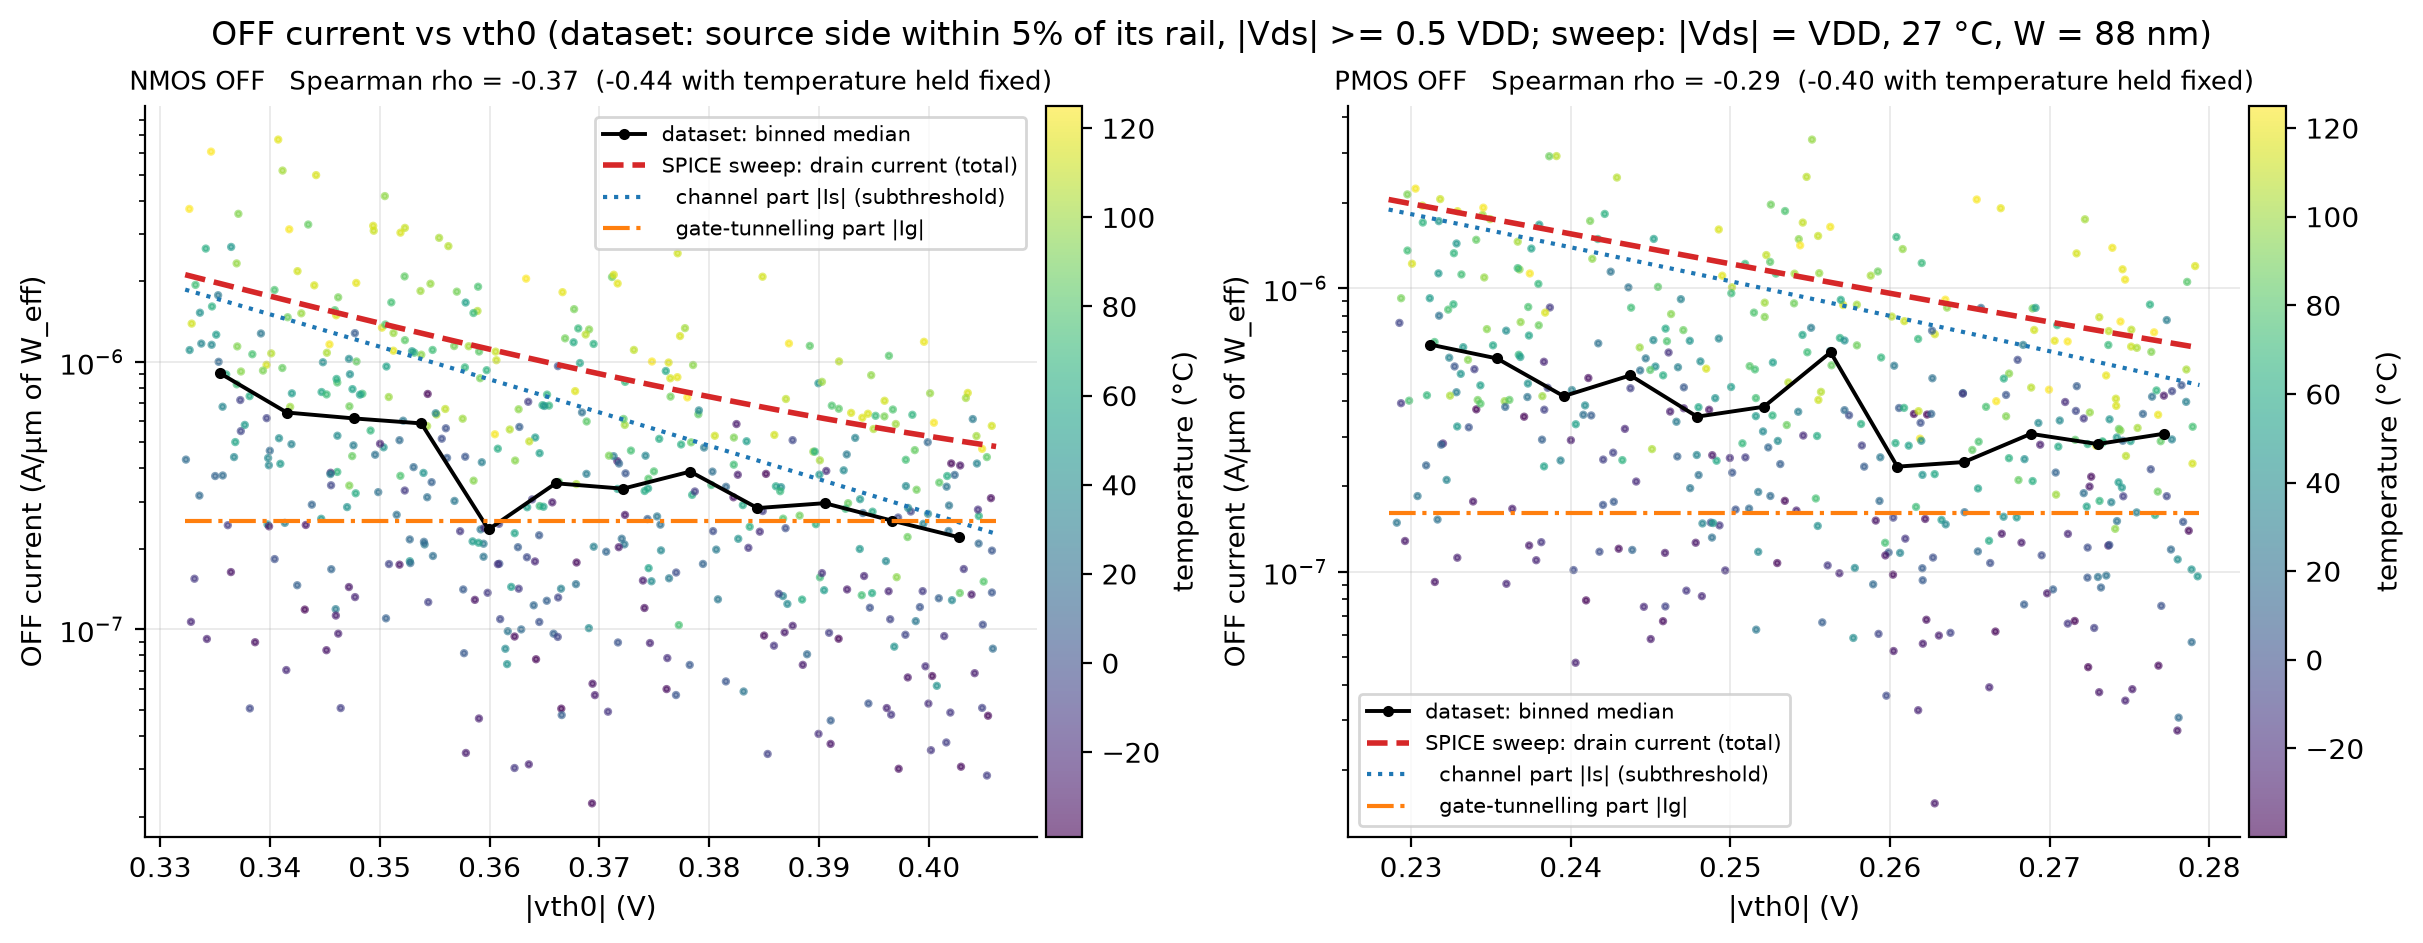
\includegraphics[width=\linewidth]{data_check/off_current_vs_vth0.png}
\caption{OFF current versus \texttt{vth0}; colour shows temperature.}
\label{fig:trend_v}
\end{figure}

\begin{figure}[H]
\centering
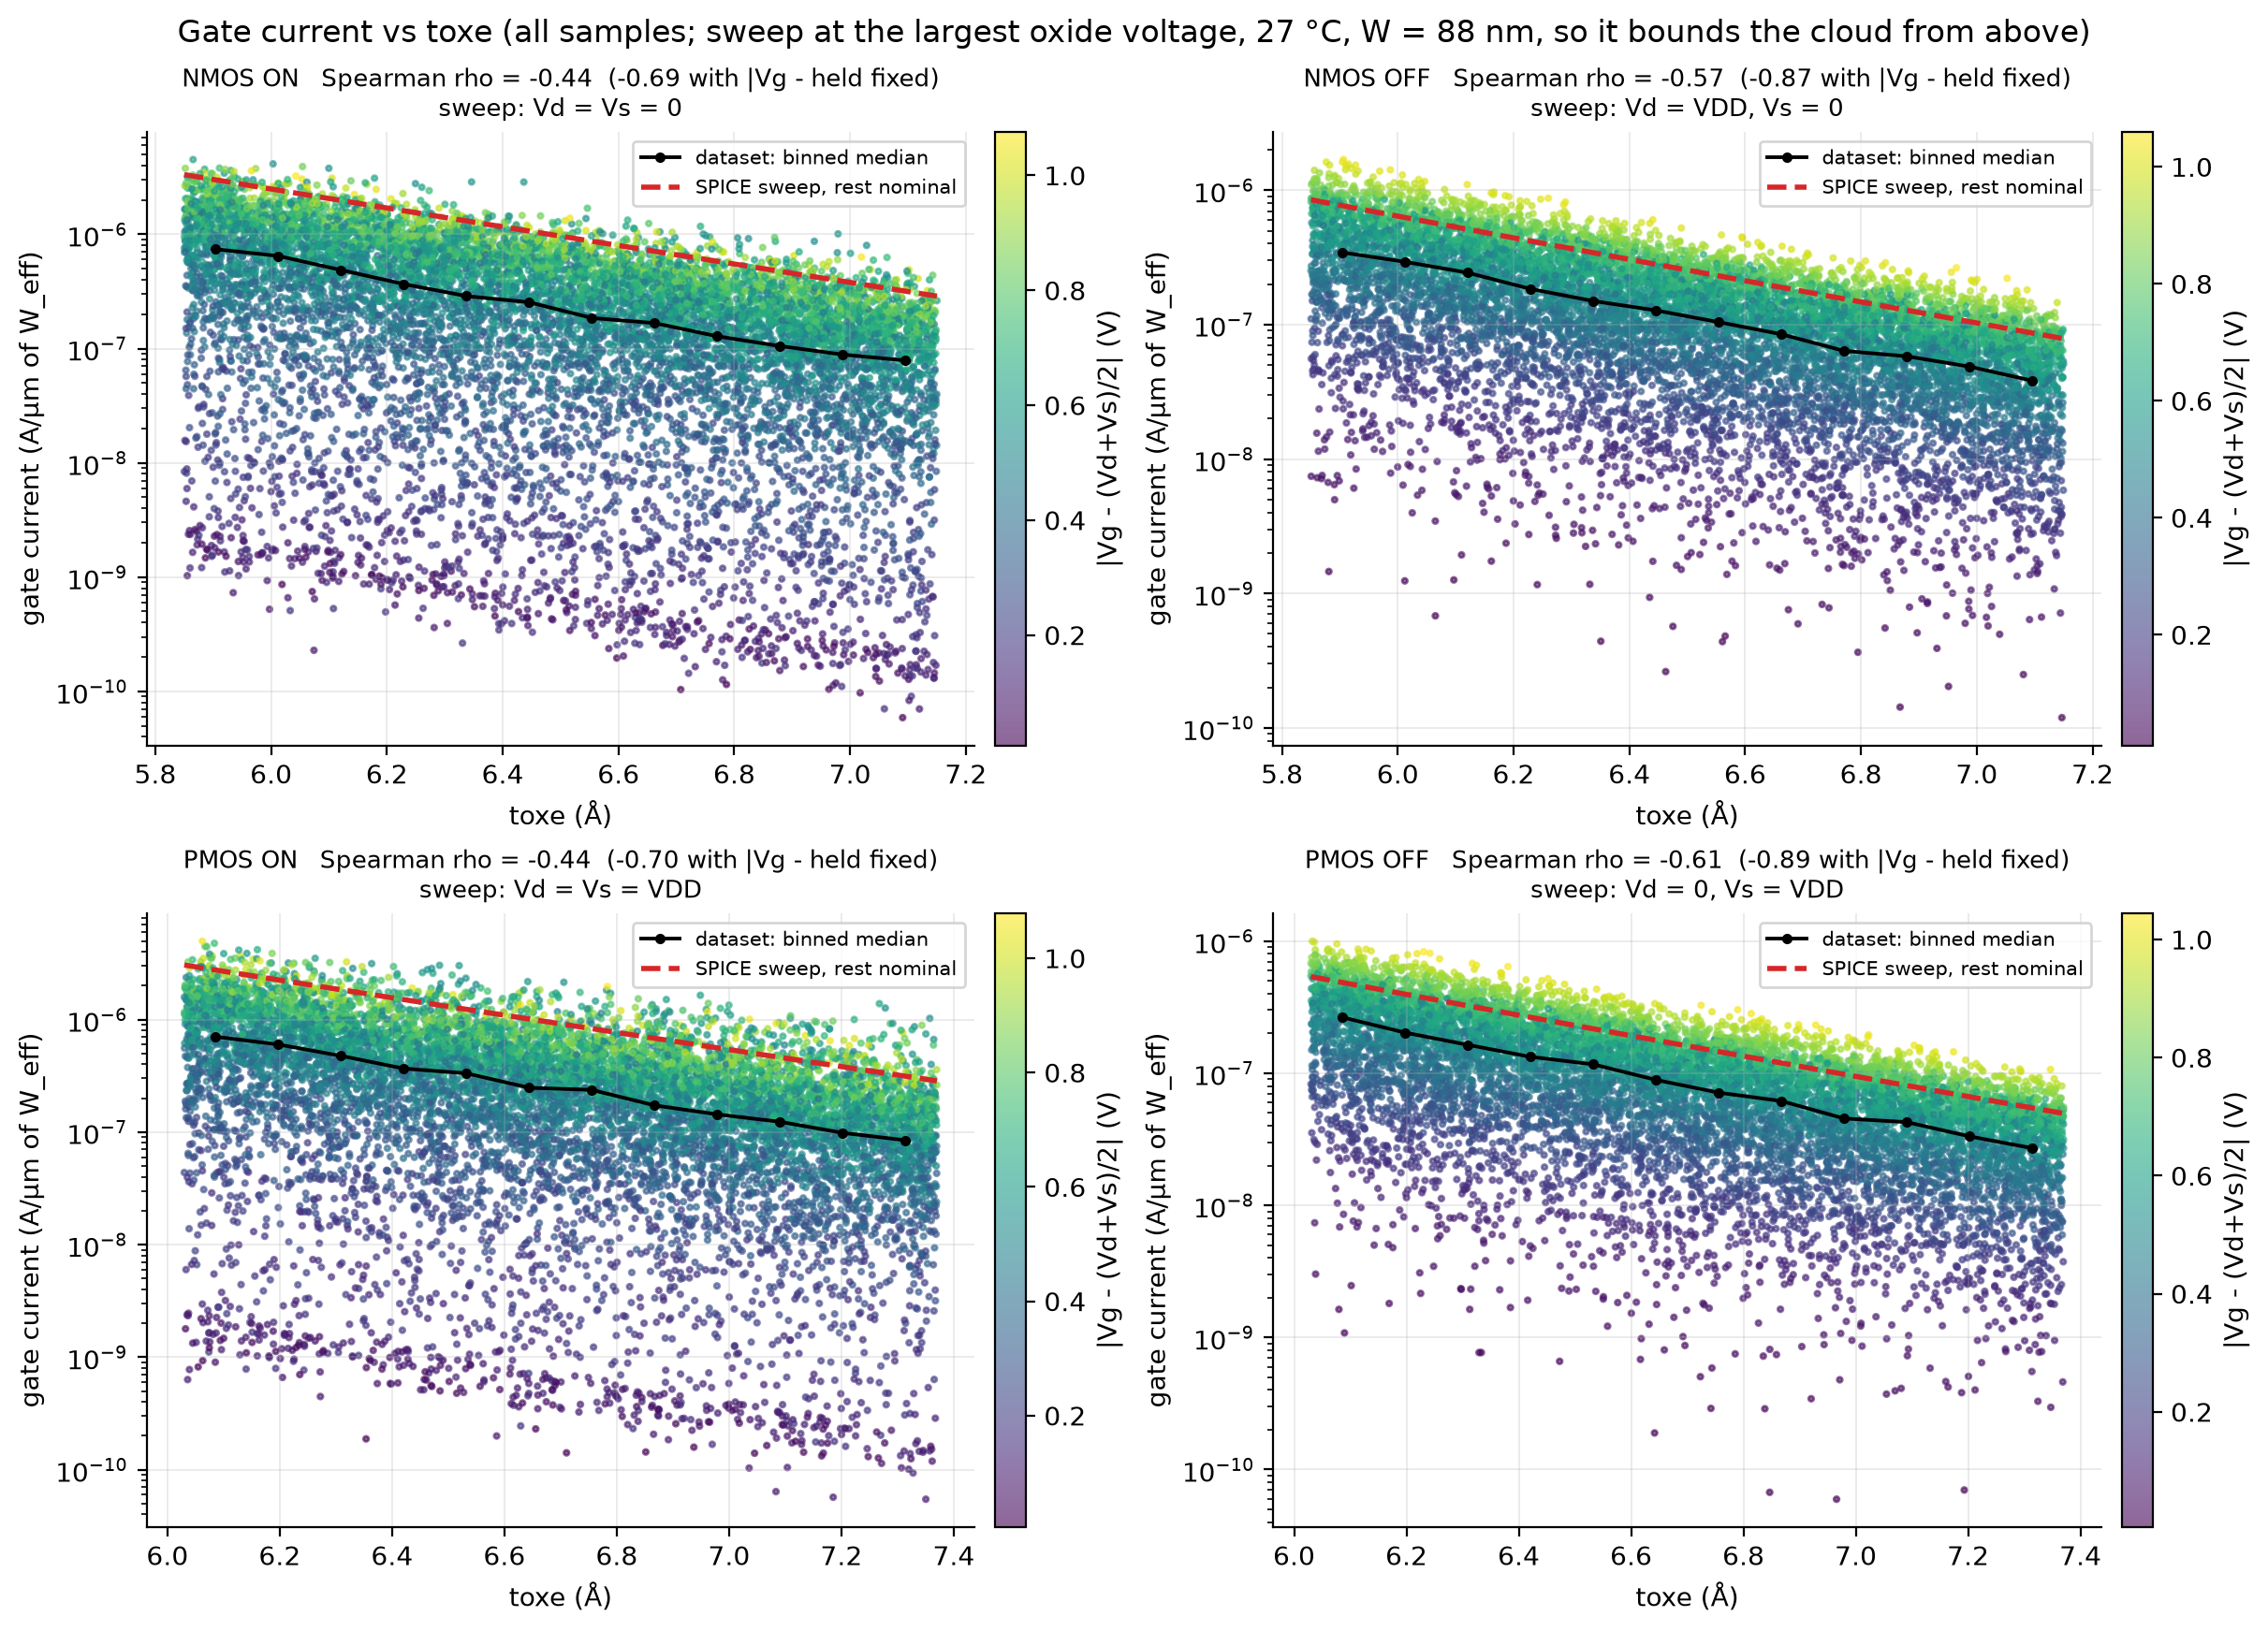
\includegraphics[width=\linewidth]{data_check/gate_current_vs_toxe.png}
\caption{Gate current versus \texttt{toxe} for all four cases; colour shows the oxide voltage.}
\label{fig:trend_tox}
\end{figure}

% ==========================================
% SECTION 3: MODELS
% ==========================================
\newpage
\addtocontents{toc}{\protect\thispagestyle{tocpage}}
\section{Models}
\label{sec:models}

\keepspace{14\baselineskip}
\subsection{Preprocessing}
\noindent Raw currents are poor targets: $I_d$ and $I_s$ change sign, and magnitudes span up to ten decades. With $J = -I$ the current into each terminal, Kirchhoff's law splits the drain and source currents exactly into a channel part $T = (J_d - J_s)/2$ and a shared part $S = -(J_g + J_b)/2$, with $J_d = T + S$ and $J_s = -T + S$. Each model predicts three smooth quantities,
\begin{equation}
    y_1 = \log_{10}\frac{T/(V_d - V_s)}{W_{\text{eff}}}, \qquad
    y_2 = \log_{10}\frac{|J_g|}{W_{\text{eff}}}, \qquad
    y_3 = \operatorname{asinh}\frac{J_b}{2 s_b},
\end{equation}

\noindent from which all four currents are rebuilt, so the predictions satisfy Kirchhoff's law exactly. Here $W_{\text{eff}} = W - 10$\,nm and $s_b$ is the body-current resolution of the simulator. The inputs are $V_{DD}$, temperature, $\ln W_{\text{eff}}$, the higher and lower of $V_d$, $V_s$ referred to the body (drain and source are interchangeable), and the five process parameters, all standardized.

\keepspace{235pt}
\subsection{Model Types and Hyperparameters}
\noindent Four model types were tried over the grids in Table~\ref{tab:grid}. Every configuration was fitted on the training set and scored on the validation set; the configuration with the lowest pooled 95th-percentile validation error was chosen.

\begin{table}[H]
\centering
\small
\begin{tabularx}{\linewidth}{|>{\raggedright\arraybackslash}p{3.6cm}|L|}
\hline
\textbf{Model type} & \textbf{Main hyperparameters (grid)} \\
\hline
Polynomial ridge & degree $\in \{2,3,4\}$; $\alpha \in \{10^{-8}, 10^{-5}, 10^{-2}\}$ \\
\hline
Random forest & 300 trees; min.\ samples per leaf $\in \{1,3\}$; max.\ features $\in \{0.5, 1.0\}$ \\
\hline
Gradient boosting & learning rate $\in \{0.05, 0.1\}$; 1000 iterations; max.\ leaf nodes $\in \{31, 63\}$ \\
\hline
Neural network (MLP) & tanh, L-BFGS, one network per target; hidden layers $\in \{64^3, 96^3\}$; $\alpha \in \{10^{-6}, 10^{-7}\}$ \\
\hline
\end{tabularx}
\caption{Model types and hyperparameter grids.}
\label{tab:grid}
\end{table}

\keepspace{333pt}
\subsection{Model Comparison}
\noindent Table~\ref{tab:compare} gives the best configuration of each type on the validation set. The neural network is best in every case on all three statistics, with about ten times lower median and 95th-percentile error than the next type, and was chosen for all four cases. The tree ensembles approximate the smooth exponential dependence on voltage and temperature with piecewise-constant steps, and the polynomials cannot follow it over several decades of current.

\begin{table}[H]
\centering
\small
\begin{tabularx}{\linewidth}{|>{\raggedright\arraybackslash}p{1.9cm}|C|C|C|C|}
\hline
\textbf{Case} & \textbf{Polynomial ridge} & \textbf{Random forest} & \textbf{Gradient boosting} & \textbf{Neural network} \\
\hline
NMOS ON & 0.9976 / 6.47 / 22.9 & 0.9817 / 15.83 / 88.7 & 0.9972 / 3.77 / 33.6 & \textbf{0.9997 / 0.45 / 2.7} \\
\hline
NMOS OFF & 0.6588 / 10.86 / 609.7 & 0.8743 / 12.21 / 100.3 & 0.9284 / 5.01 / 99.8 & \textbf{0.9855 / 0.46 / 19.9} \\
\hline
PMOS ON & 0.9963 / 3.89 / 20.9 & 0.9848 / 10.90 / 77.3 & 0.9969 / 2.99 / 30.0 & \textbf{0.9999 / 0.37 / 2.1} \\
\hline
PMOS OFF & 0.9434 / 4.23 / 117.6 & 0.9425 / 7.84 / 76.2 & 0.9866 / 2.89 / 33.9 & \textbf{0.9994 / 0.32 / 4.7} \\
\hline
\end{tabularx}
\caption{Model comparison on the validation set: $R^2$ of $\log_{10}|I|$ / median error (\%) / 95th-percentile error (\%), pooled over the four currents. Bold: chosen model.}
\label{tab:compare}
\end{table}

\keepspace{281pt}
\subsection{Chosen Models}
\noindent The chosen networks are $64\times64\times64$ for NMOS ON ($\alpha = 10^{-6}$), NMOS OFF and PMOS ON ($\alpha = 10^{-7}$), and $96\times96\times96$ for PMOS OFF ($\alpha = 10^{-6}$); the differences between network configurations were below 10\,\% in validation p95. Table~\ref{tab:chosen} gives their test-set errors and Figure~\ref{fig:pvs} the predicted-versus-SPICE plots. $R^2$ of $\log_{10}|I|$ exceeds 0.994 for every current except the NMOS OFF body current (0.962), which changes sign around $10^{-17}$\,A and dominates the pooled NMOS OFF tail.

\begin{table}[H]
\centering
\small
\begin{tabularx}{\linewidth}{|>{\raggedright\arraybackslash}p{1.9cm}|c|C|C|C|C|}
\hline
\textbf{Case} & \textbf{Pooled} & \textbf{$I_d$} & \textbf{$I_g$} & \textbf{$I_s$} & \textbf{$I_b$} \\
\hline
NMOS ON & 0.46 / 2.75 & 0.45 / 2.6 & 0.36 / 4.0 & 0.45 / 2.5 & 0.61 / 2.7 \\
\hline
NMOS OFF & 0.44 / 20.02 & 0.35 / 6.0 & 0.22 / 1.0 & 0.32 / 4.9 & 5.79 / 84.9 \\
\hline
PMOS ON & 0.36 / 2.18 & 0.28 / 1.8 & 0.39 / 2.6 & 0.28 / 1.8 & 0.60 / 2.6 \\
\hline
PMOS OFF & 0.34 / 4.90 & 0.35 / 5.2 & 0.24 / 1.0 & 0.33 / 4.7 & 1.75 / 9.4 \\
\hline
\end{tabularx}
\caption{Chosen models on the test set: median / 95th-percentile relative error (\%).}
\label{tab:chosen}
\end{table}

\begin{figure}[H]
\centering
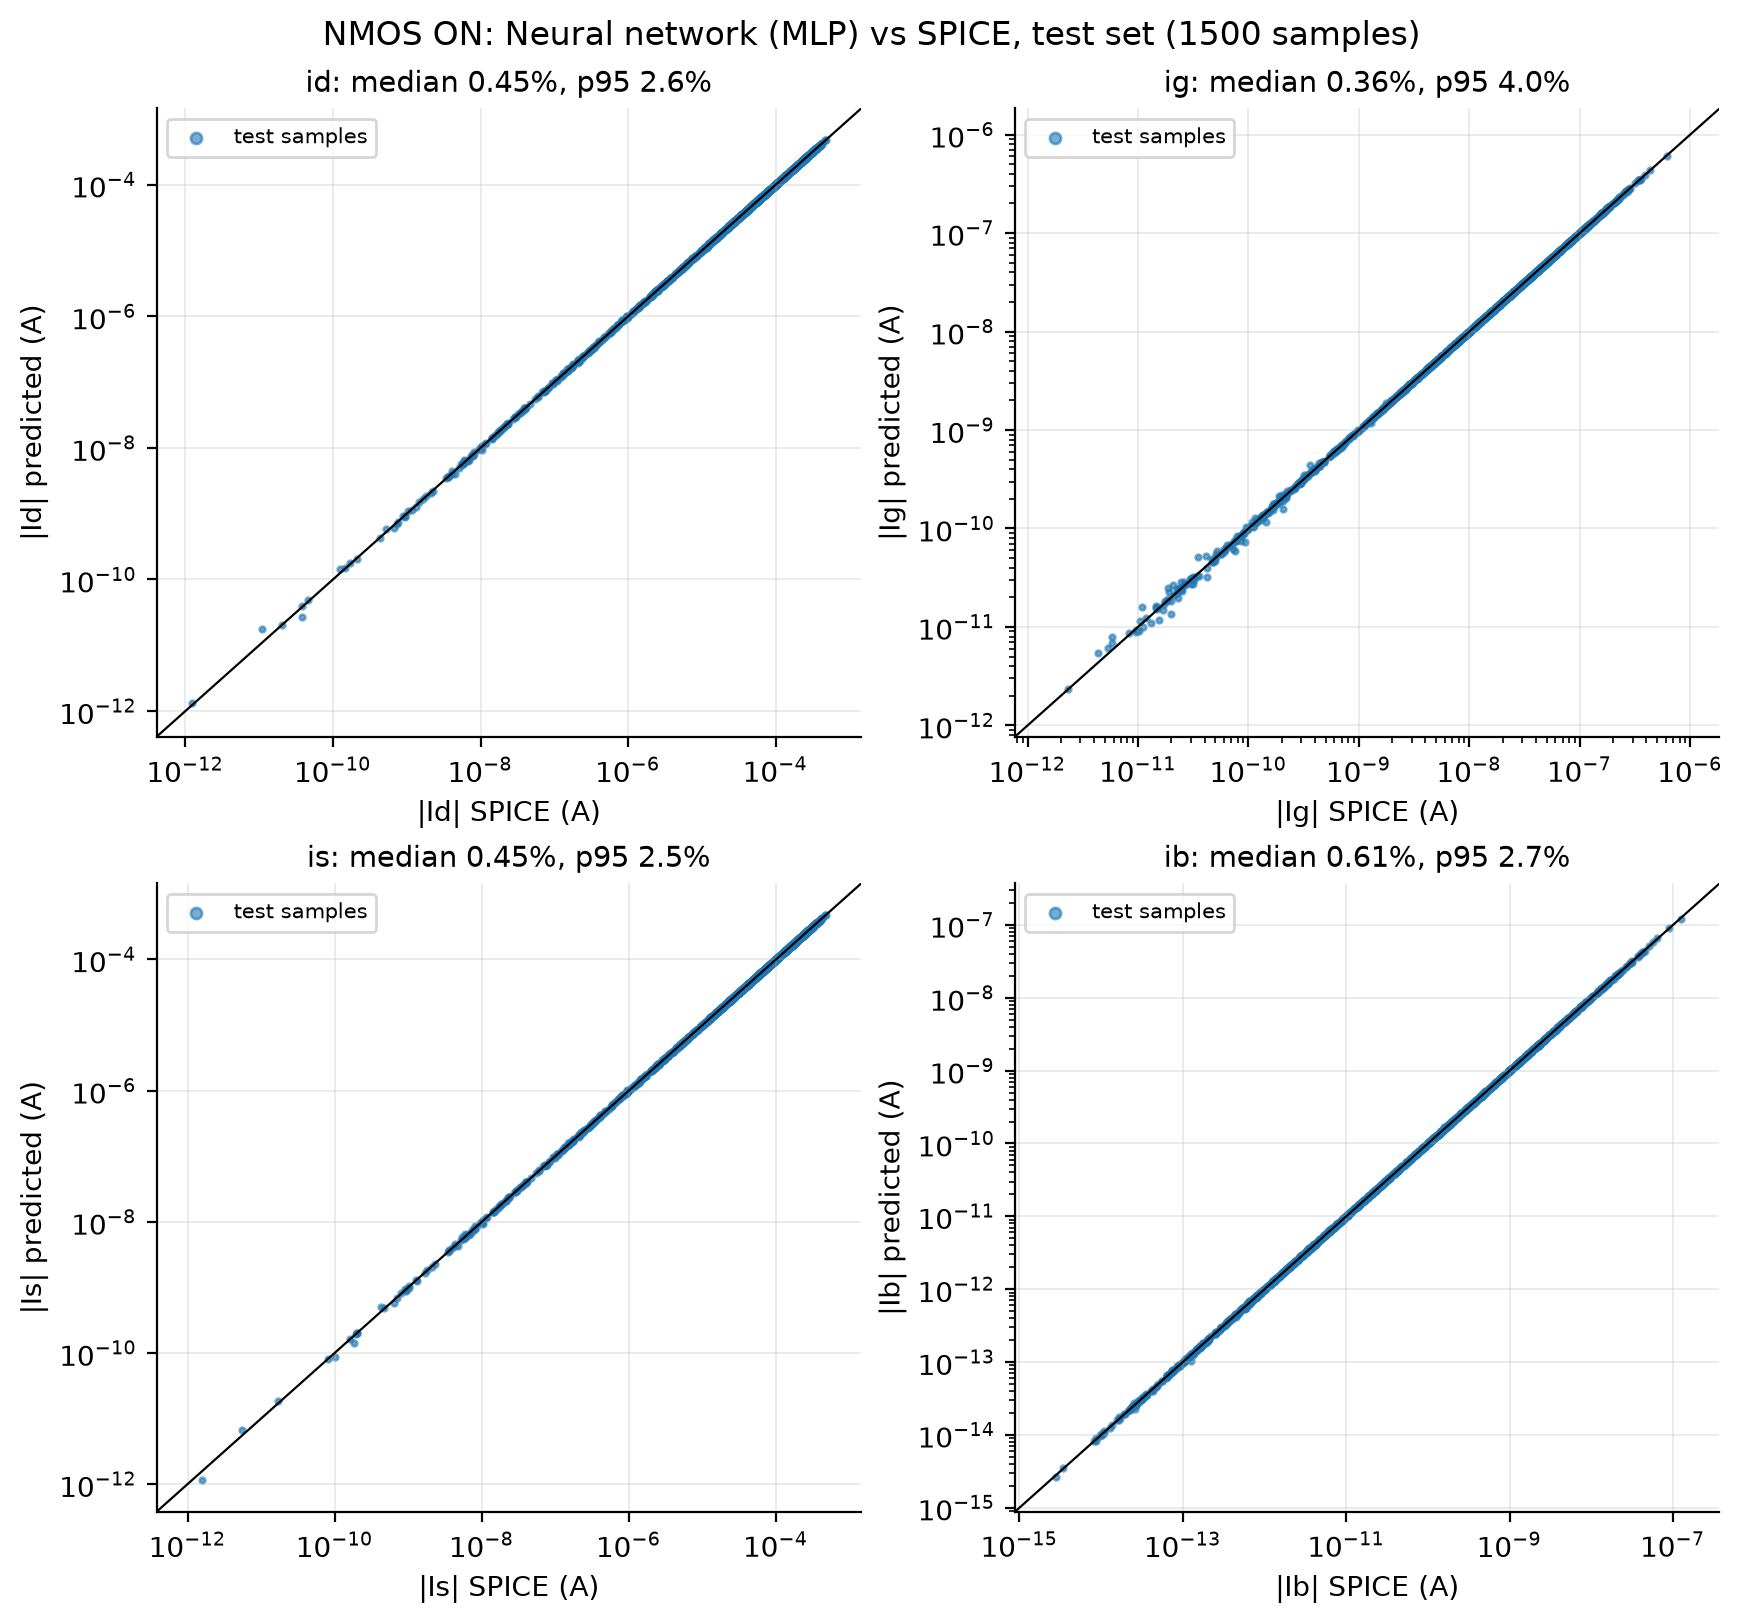
\includegraphics[width=0.49\linewidth]{model_selection/pred_vs_spice_nmos_on.png}
\hfill
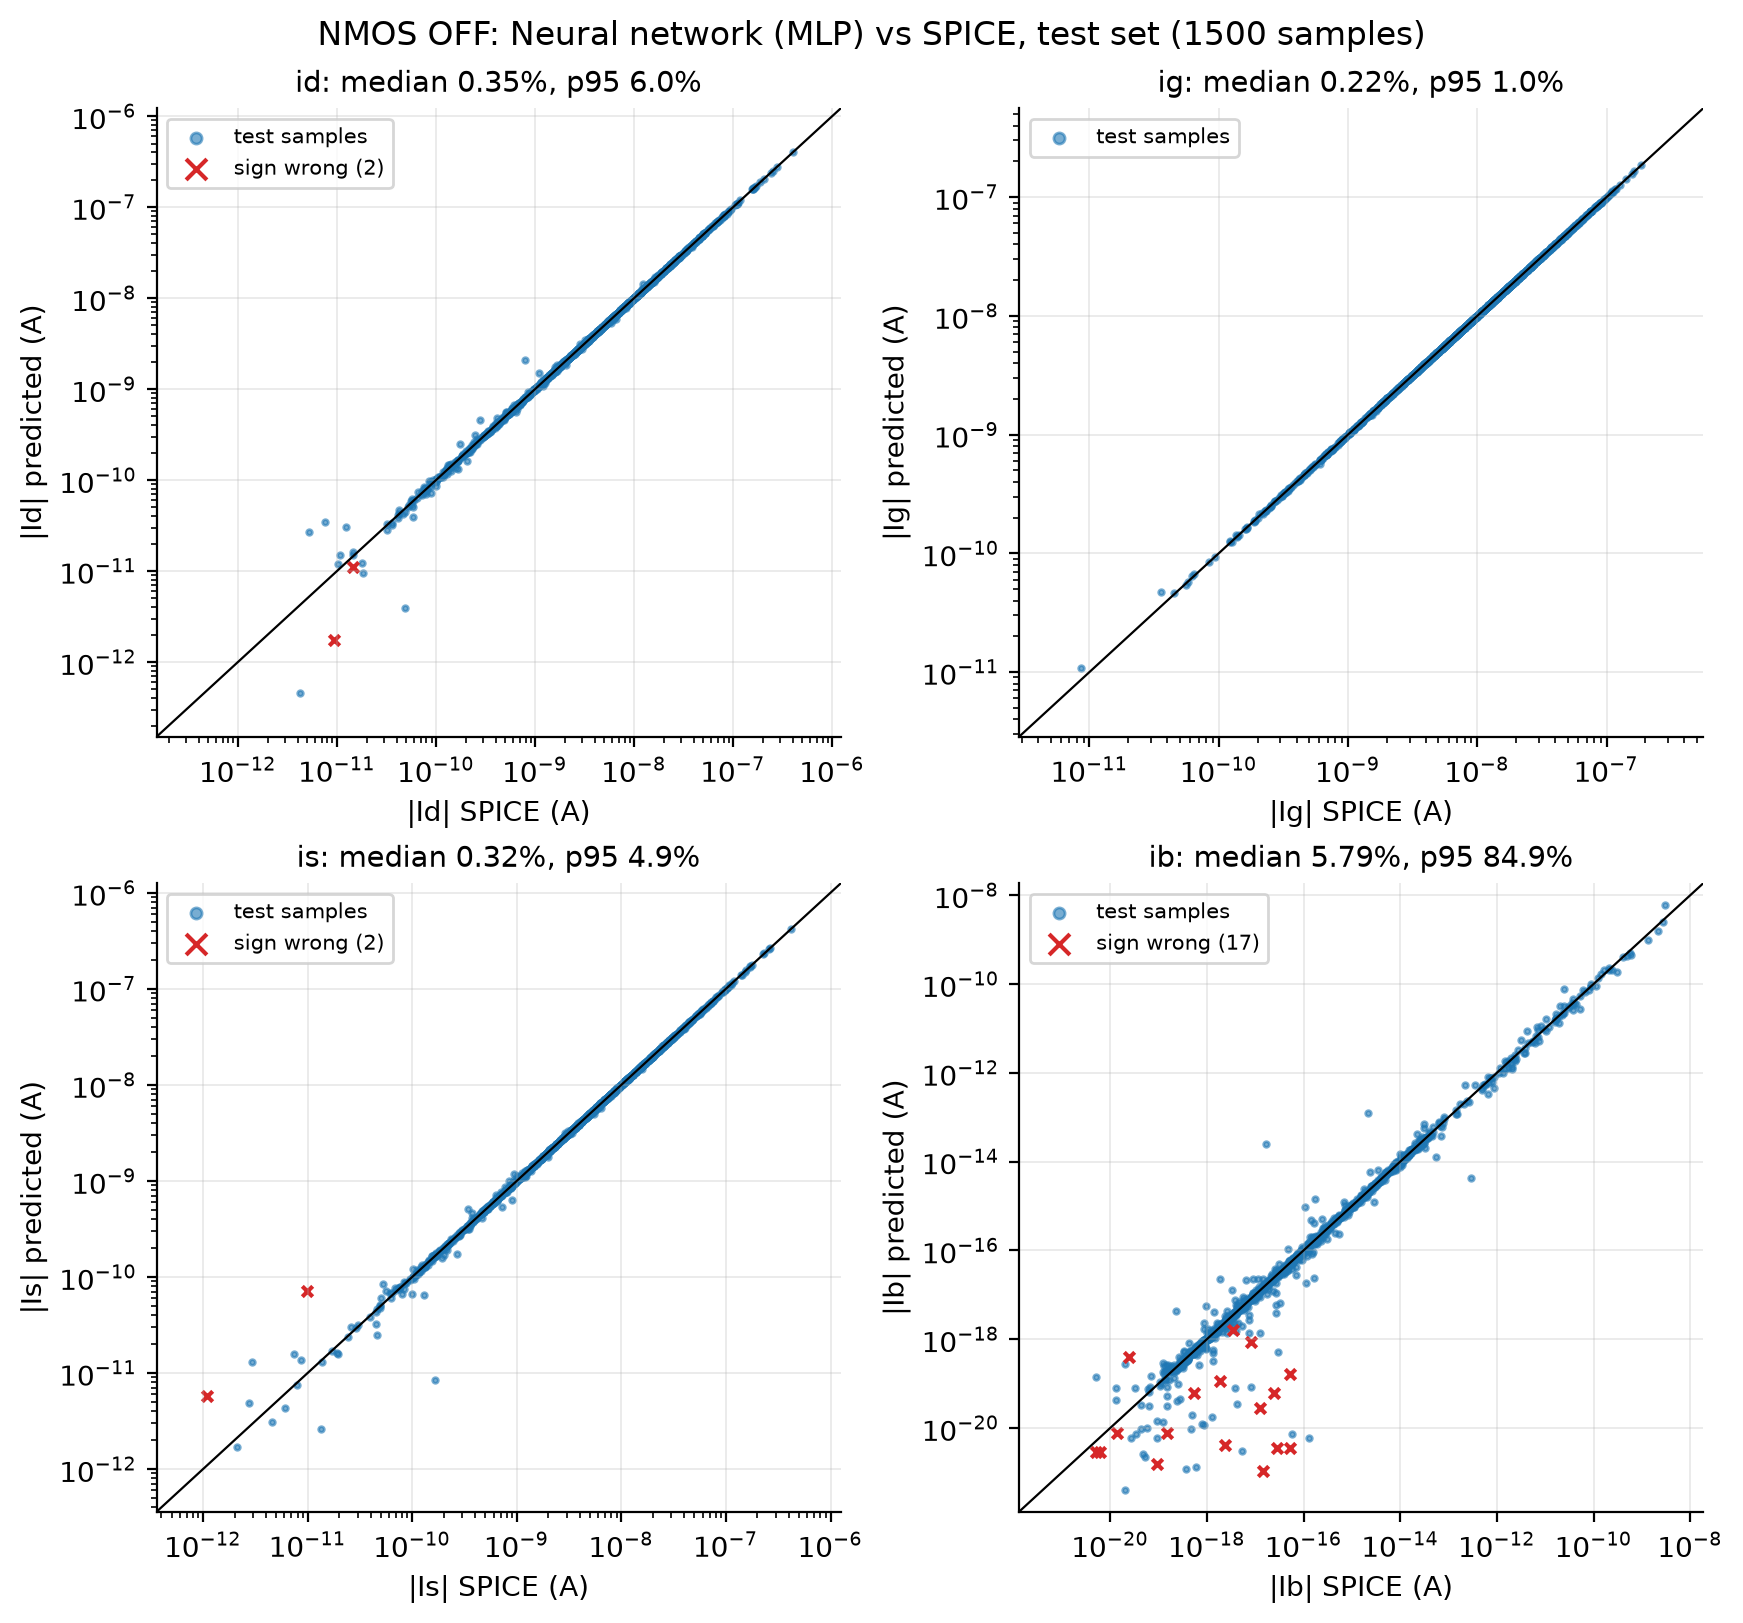
\includegraphics[width=0.49\linewidth]{model_selection/pred_vs_spice_nmos_off.png}

\vspace{0.3cm}
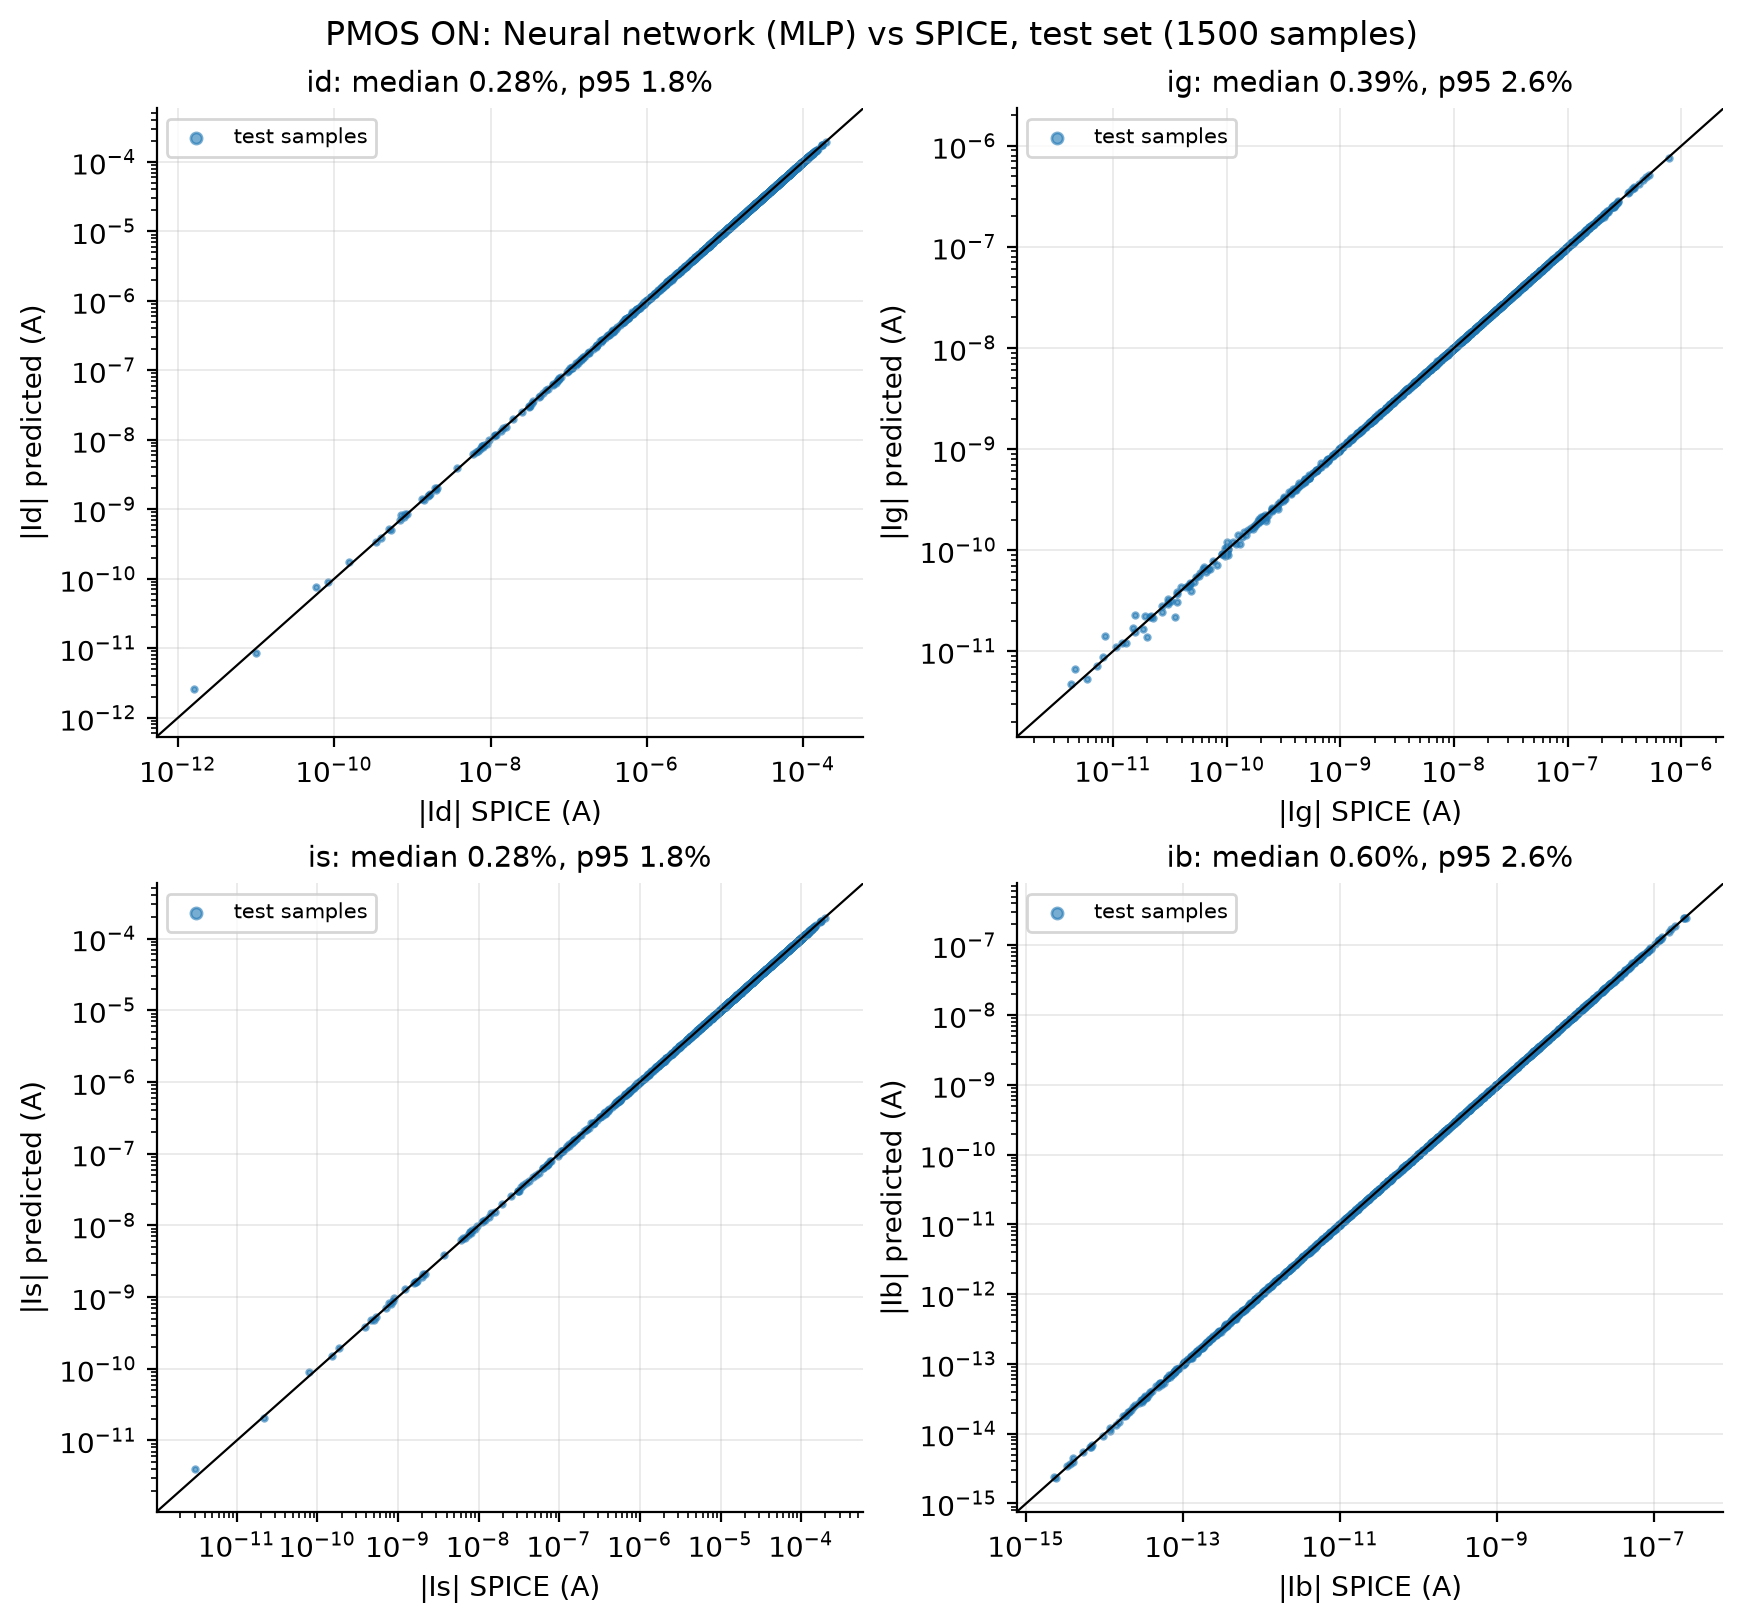
\includegraphics[width=0.49\linewidth]{model_selection/pred_vs_spice_pmos_on.png}
\hfill
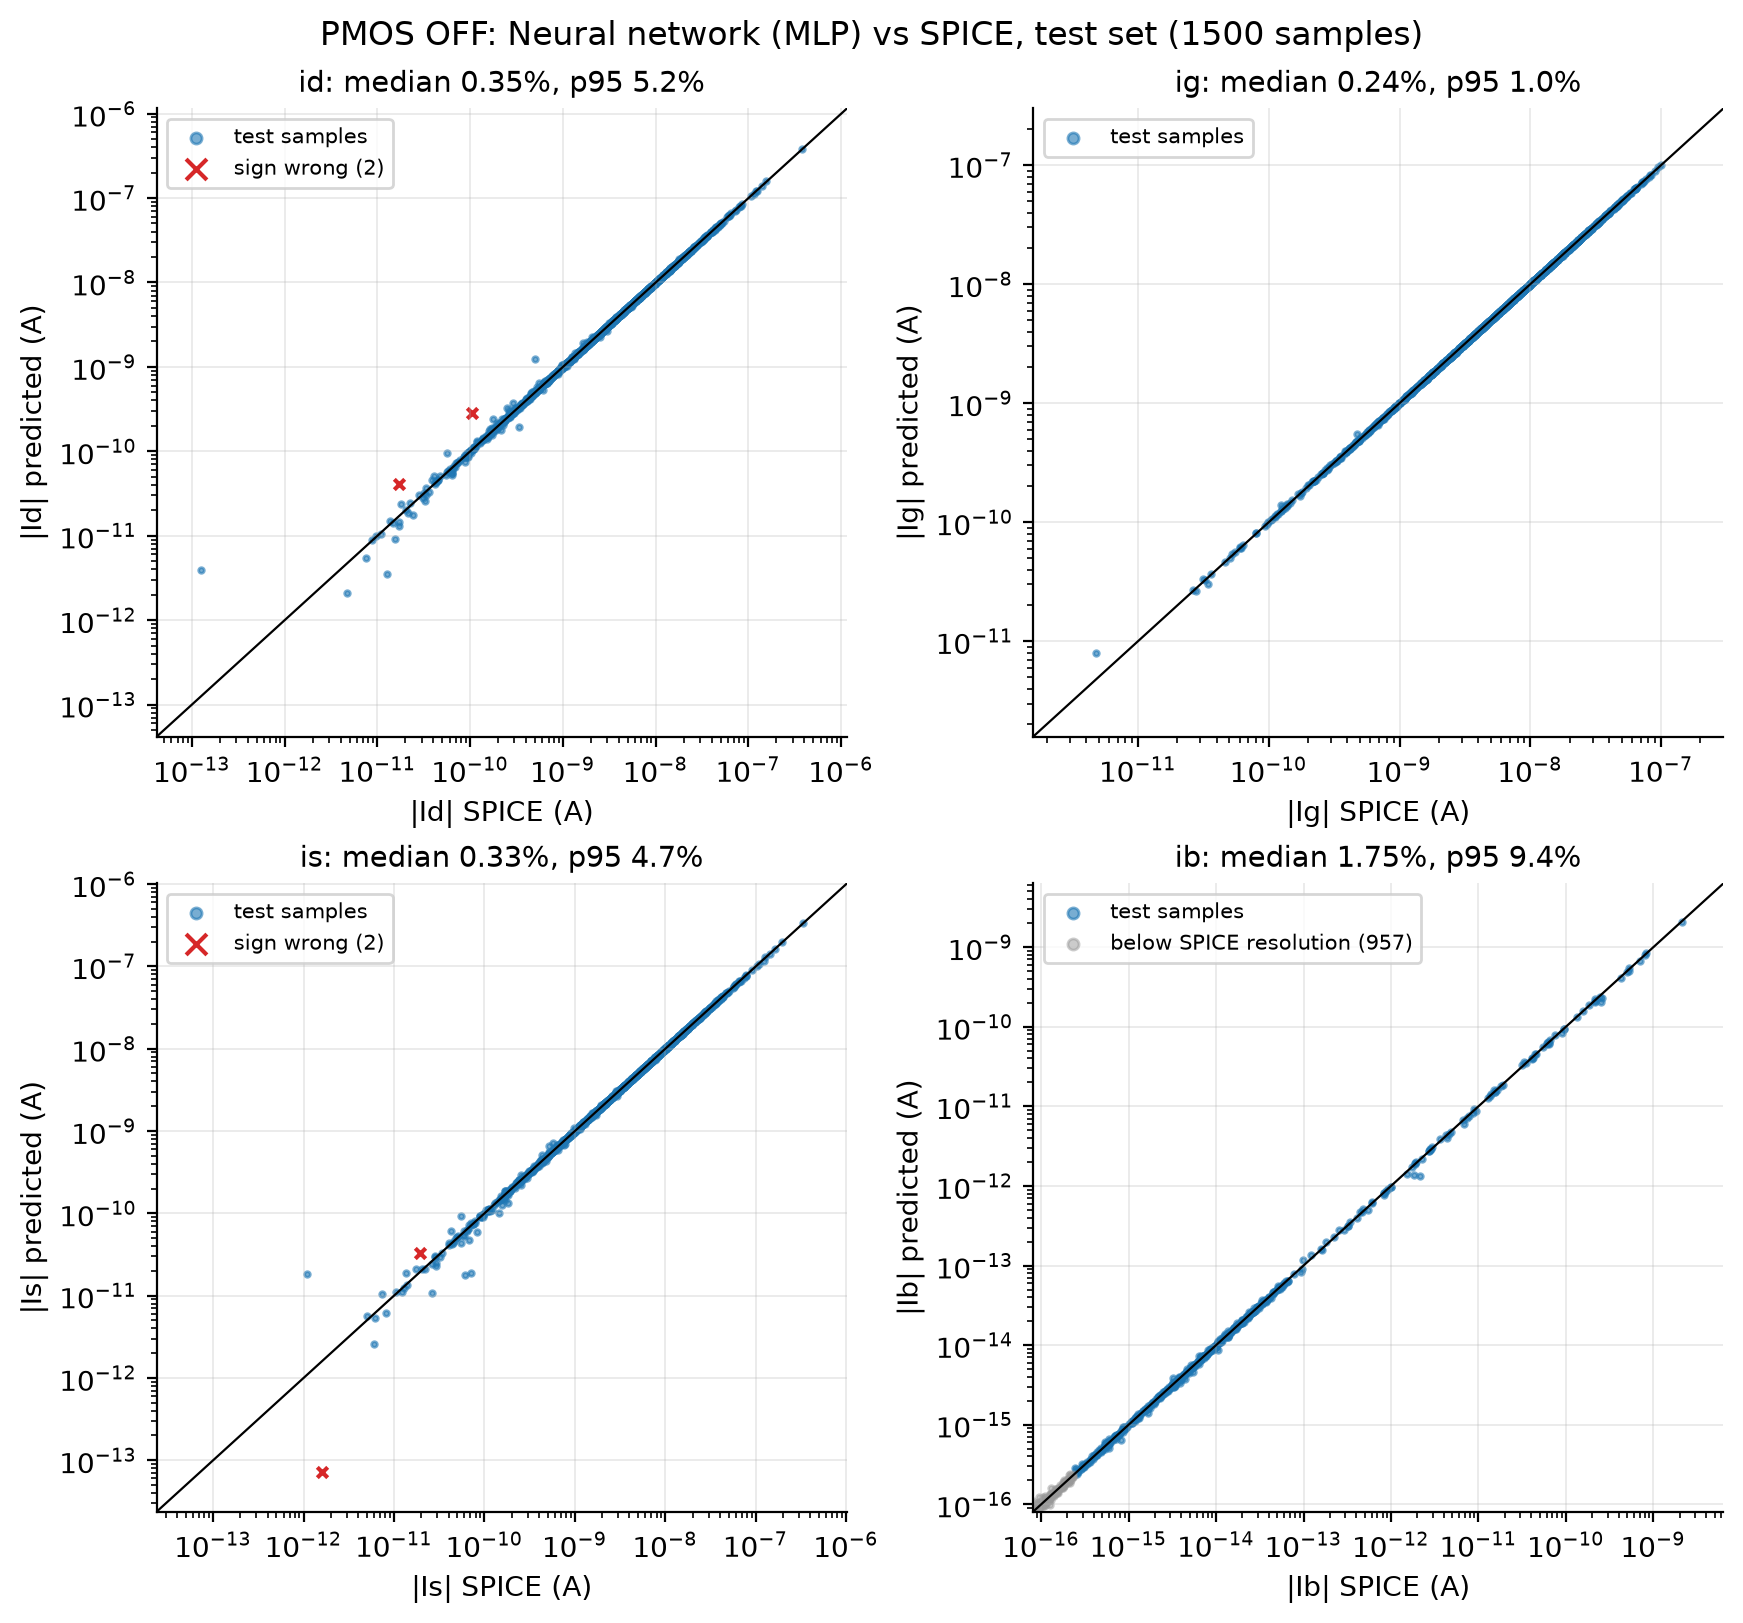
\includegraphics[width=0.49\linewidth]{model_selection/pred_vs_spice_pmos_off.png}
\caption{Predicted versus SPICE terminal currents on the test set: NMOS ON, NMOS OFF (top); PMOS ON, PMOS OFF (bottom).}
\label{fig:pvs}
\end{figure}

\keepspace{361pt}
\subsection{Improved Models}
\label{sec:improved}
\noindent The validation error still fell at the largest training-set size (from 4,000 to 7,000 samples: $-8$ to $-21\,\%$ in median), so the chosen networks were improved in two steps. \textbf{v2} trains each on 27,000 uniform samples and averages five networks trained from different random starts. \textbf{v3} adds 7,000 rail-focused samples and seven physics features ($1000/T$, junction reverse-bias terms, $\tanh(V_{ds}/V_t)$ and the log gate-to-diffusion voltages). The original models are referred to as \textbf{v1}. Table~\ref{tab:v123} compares the three versions on the uniform test set and on the rail-focused test set, which mimics the operating points inside gates.

\begin{table}[H]
\centering
\small
\begin{tabularx}{\linewidth}{|>{\raggedright\arraybackslash}p{1.9cm}|>{\raggedright\arraybackslash}p{1.3cm}|C|C|C|}
\hline
\textbf{Case} & \textbf{Test set} & \textbf{v1} & \textbf{v2} & \textbf{v3} \\
\hline
\multirow{2}{1.9cm}{NMOS ON} & uniform & 0.46 / 2.75 & 0.27 / 1.76 & 0.30 / \textbf{1.65} \\
\cline{2-5}
 & rail & 0.62 / 10.34 & 0.36 / 5.38 & 0.39 / \textbf{2.49} \\
\hline
\multirow{2}{1.9cm}{NMOS OFF} & uniform & 0.44 / 20.02 & 0.25 / 7.25 & 0.26 / \textbf{6.51} \\
\cline{2-5}
 & rail & 0.90 / 79.61 & 0.53 / 30.25 & \textbf{0.43} / \textbf{9.98} \\
\hline
\multirow{2}{1.9cm}{PMOS ON} & uniform & 0.36 / 2.18 & 0.21 / 1.51 & 0.21 / \textbf{1.23} \\
\cline{2-5}
 & rail & 0.51 / 7.91 & 0.29 / 5.76 & \textbf{0.28} / \textbf{2.11} \\
\hline
\multirow{2}{1.9cm}{PMOS OFF} & uniform & 0.34 / 4.90 & 0.17 / 2.54 & 0.21 / 2.56 \\
\cline{2-5}
 & rail & 0.69 / 16.96 & 0.37 / 10.98 & \textbf{0.31} / \textbf{3.72} \\
\hline
\end{tabularx}
\caption{Transistor models of the three versions: pooled median / 95th-percentile test error (\%). Bold: best version.}
\label{tab:v123}
\end{table}

\noindent On uniform samples v2 and v3 are equally accurate; on rail-focused samples v3 cuts the 95th-percentile error four- to eightfold relative to v1, most of all for the ON-state gate current (NMOS ON: 58.9\,\% in v1, 2.9\,\% in v3). For v3, $R^2$ exceeds 0.99 for every current of every case. The v3 models are used for the final gate and test-circuit results.

% ==========================================
% SECTION 4: GATE RESULTS
% ==========================================
\newpage
\addtocontents{toc}{\protect\thispagestyle{tocpage}}
\section{Gate Results}
\label{sec:gates}

\keepspace{14\baselineskip}
\subsection{Method}
\noindent The gates are static CMOS with $W_n/W_p$ of 44/88\,nm (INV), 88/88\,nm (NAND2) and 44/176\,nm (NOR2); AND2 and OR2 are a NAND2 or NOR2 followed by an inverter and are simulated as complete gates. Every gate is simulated in SPICE at each input combination (18 cases) and at the same 200 random PVT corners (3,600 operating points), with inputs at exactly 0 or $V_{DD}$. All NMOS in a circuit share one process draw and all PMOS another.

\medskip
\noindent For the ML estimate, each transistor's drain and source voltages are taken from the recorded SPICE node voltages and its gate is at the logic rail of its node; the four models give its terminal currents. The leakage is then the current delivered by the sources of interest, obtained from Kirchhoff's law as the net current leaving the set of nodes $H$ connected to those sources through ON transistors:
\begin{equation}
    I_{\text{leak}} \;=\; \sum_{k} \;\sum_{t \in \{d,g,s,b\},\; n_{k,t} \in H} J_{k,t}.
    \label{eq:nodeset}
\end{equation}

\noindent Two definitions are reported: the \textbf{total} leakage, delivered by every source at $V_{DD}$ (the supply and the inputs at logic 1, equal to the static power divided by $V_{DD}$), and the \textbf{supply-only} leakage, delivered by $V_{DD}$ alone. With exact single-transistor SPICE currents in place of the models, Eq.~\eqref{eq:nodeset} reproduces the gate SPICE leakage to within $10^{-7}$ for INV, NAND2 and NOR2. For AND2 and OR2 the inverter's gate sits up to 7\,mV from its rail, which the models do not represent; this \emph{composition floor} is a median error of 0.08--0.67\,\% even with exact currents.

\keepspace{294pt}
\subsection{Results}
\noindent Table~\ref{tab:gsum} summarizes all 3,600 operating points for the three model versions. With v3 the mean accuracy is 99.48\,\% (total) and 99.41\,\% (supply-only), and no operating point is worse than 3.6\,\% (total). Table~\ref{tab:g3} gives the per-case results and Figure~\ref{fig:gparity} the parity plot.

\begin{table}[H]
\centering
\small
\begin{tabularx}{\linewidth}{|>{\raggedright\arraybackslash}p{2.3cm}|c|C|C|C|C|C|c|}
\hline
\textbf{Leakage} & \textbf{Version} & \textbf{Median err.} & \textbf{p95 err.} & \textbf{Mean err.} & \textbf{Mean accuracy} & \textbf{Bias} & \textbf{Max err.} \\
\hline
\multirow{3}{2.3cm}{Total} & v1 & 0.71 & 3.47 & 1.09 & 98.91 & $-0.59$ & 25.7 \\
\cline{2-8}
 & v2 & 0.42 & 1.63 & 0.58 & 99.42 & $-0.35$ & 5.0 \\
\cline{2-8}
 & v3 & \textbf{0.40} & \textbf{1.46} & \textbf{0.52} & \textbf{99.48} & $\mathbf{-0.23}$ & \textbf{3.6} \\
\hline
\multirow{3}{2.3cm}{Supply only} & v1 & 0.94 & 4.60 & 1.44 & 98.56 & $-0.59$ & 25.7 \\
\cline{2-8}
 & v2 & 0.57 & 2.04 & 0.76 & 99.24 & $-0.41$ & 7.2 \\
\cline{2-8}
 & v3 & \textbf{0.48} & \textbf{1.54} & \textbf{0.59} & \textbf{99.41} & $\mathbf{-0.28}$ & \textbf{6.2} \\
\hline
\end{tabularx}
\caption{Gate leakage over all 18 cases and 200 corners: errors (\%) of the three model versions.}
\label{tab:gsum}
\end{table}

\begin{table}[H]
\centering
\scriptsize
\begin{tabularx}{\linewidth}{|>{\raggedright\arraybackslash}p{1.0cm}|c|C|C|C|C|C|C|}
\hline
\textbf{Gate} & \textbf{AB} & \textbf{SPICE median (nA)} & \textbf{ML median (nA)} & \textbf{Bias (\%)} & \textbf{Median err. (\%)} & \textbf{p95 err. (\%)} & \textbf{Supply-only median err. / p95 (\%)} \\
\hline
INV & 0 & 134.85 & 136.50 & $+0.33$ & 0.50 & 1.47 & 0.50 / 1.47 \\
\hline
INV & 1 & 156.49 & 156.49 & $+0.09$ & 0.22 & 0.73 & 0.30 / 1.00 \\
\hline
NAND2 & 00 & 170.20 & 169.98 & $+0.11$ & 0.52 & 1.43 & 0.52 / 1.43 \\
\hline
NAND2 & 01 & 146.35 & 147.48 & $-0.24$ & 0.41 & 1.04 & 0.41 / 1.05 \\
\hline
NAND2 & 10 & 311.11 & 312.29 & $-0.15$ & 0.30 & 0.91 & 0.42 / 1.06 \\
\hline
NAND2 & 11 & 437.51 & 435.70 & $-0.08$ & 0.24 & 0.88 & 0.30 / 1.00 \\
\hline
NOR2 & 00 & 457.67 & 457.26 & $-0.08$ & 0.47 & 1.46 & 0.47 / 1.46 \\
\hline
NOR2 & 01 & 459.76 & 459.27 & $-0.29$ & 0.39 & 1.14 & 0.45 / 1.21 \\
\hline
NOR2 & 10 & 186.07 & 185.15 & $-0.26$ & 0.35 & 0.81 & 0.53 / 1.21 \\
\hline
NOR2 & 11 & 120.92 & 121.29 & $-0.11$ & 0.40 & 1.16 & 0.66 / 1.48 \\
\hline
AND2 & 00 & 362.79 & 362.60 & $-0.24$ & 0.37 & 1.14 & 0.37 / 1.14 \\
\hline
AND2 & 01 & 310.59 & 308.03 & $-0.88$ & 0.88 & 2.07 & 0.88 / 2.07 \\
\hline
AND2 & 10 & 472.99 & 470.38 & $-0.87$ & 0.78 & 2.13 & 1.04 / 2.34 \\
\hline
AND2 & 11 & 582.98 & 582.72 & $-0.16$ & 0.28 & 0.84 & 0.33 / 1.16 \\
\hline
OR2 & 00 & 618.13 & 615.66 & $-0.86$ & 0.79 & 2.26 & 0.79 / 2.26 \\
\hline
OR2 & 01 & 610.18 & 609.99 & $-0.33$ & 0.45 & 1.06 & 0.52 / 1.17 \\
\hline
OR2 & 10 & 325.69 & 323.97 & $-0.22$ & 0.35 & 0.87 & 0.43 / 0.96 \\
\hline
OR2 & 11 & 262.54 & 264.15 & $+0.10$ & 0.26 & 0.97 & 0.38 / 1.21 \\
\hline
\end{tabularx}
\caption{Gate results (v3) for the 18 gate and input cases over 200 corners: total leakage, with the median and 95th-percentile error of the supply-only leakage in the last column.}
\label{tab:g3}
\end{table}

\begin{figure}[H]
\centering
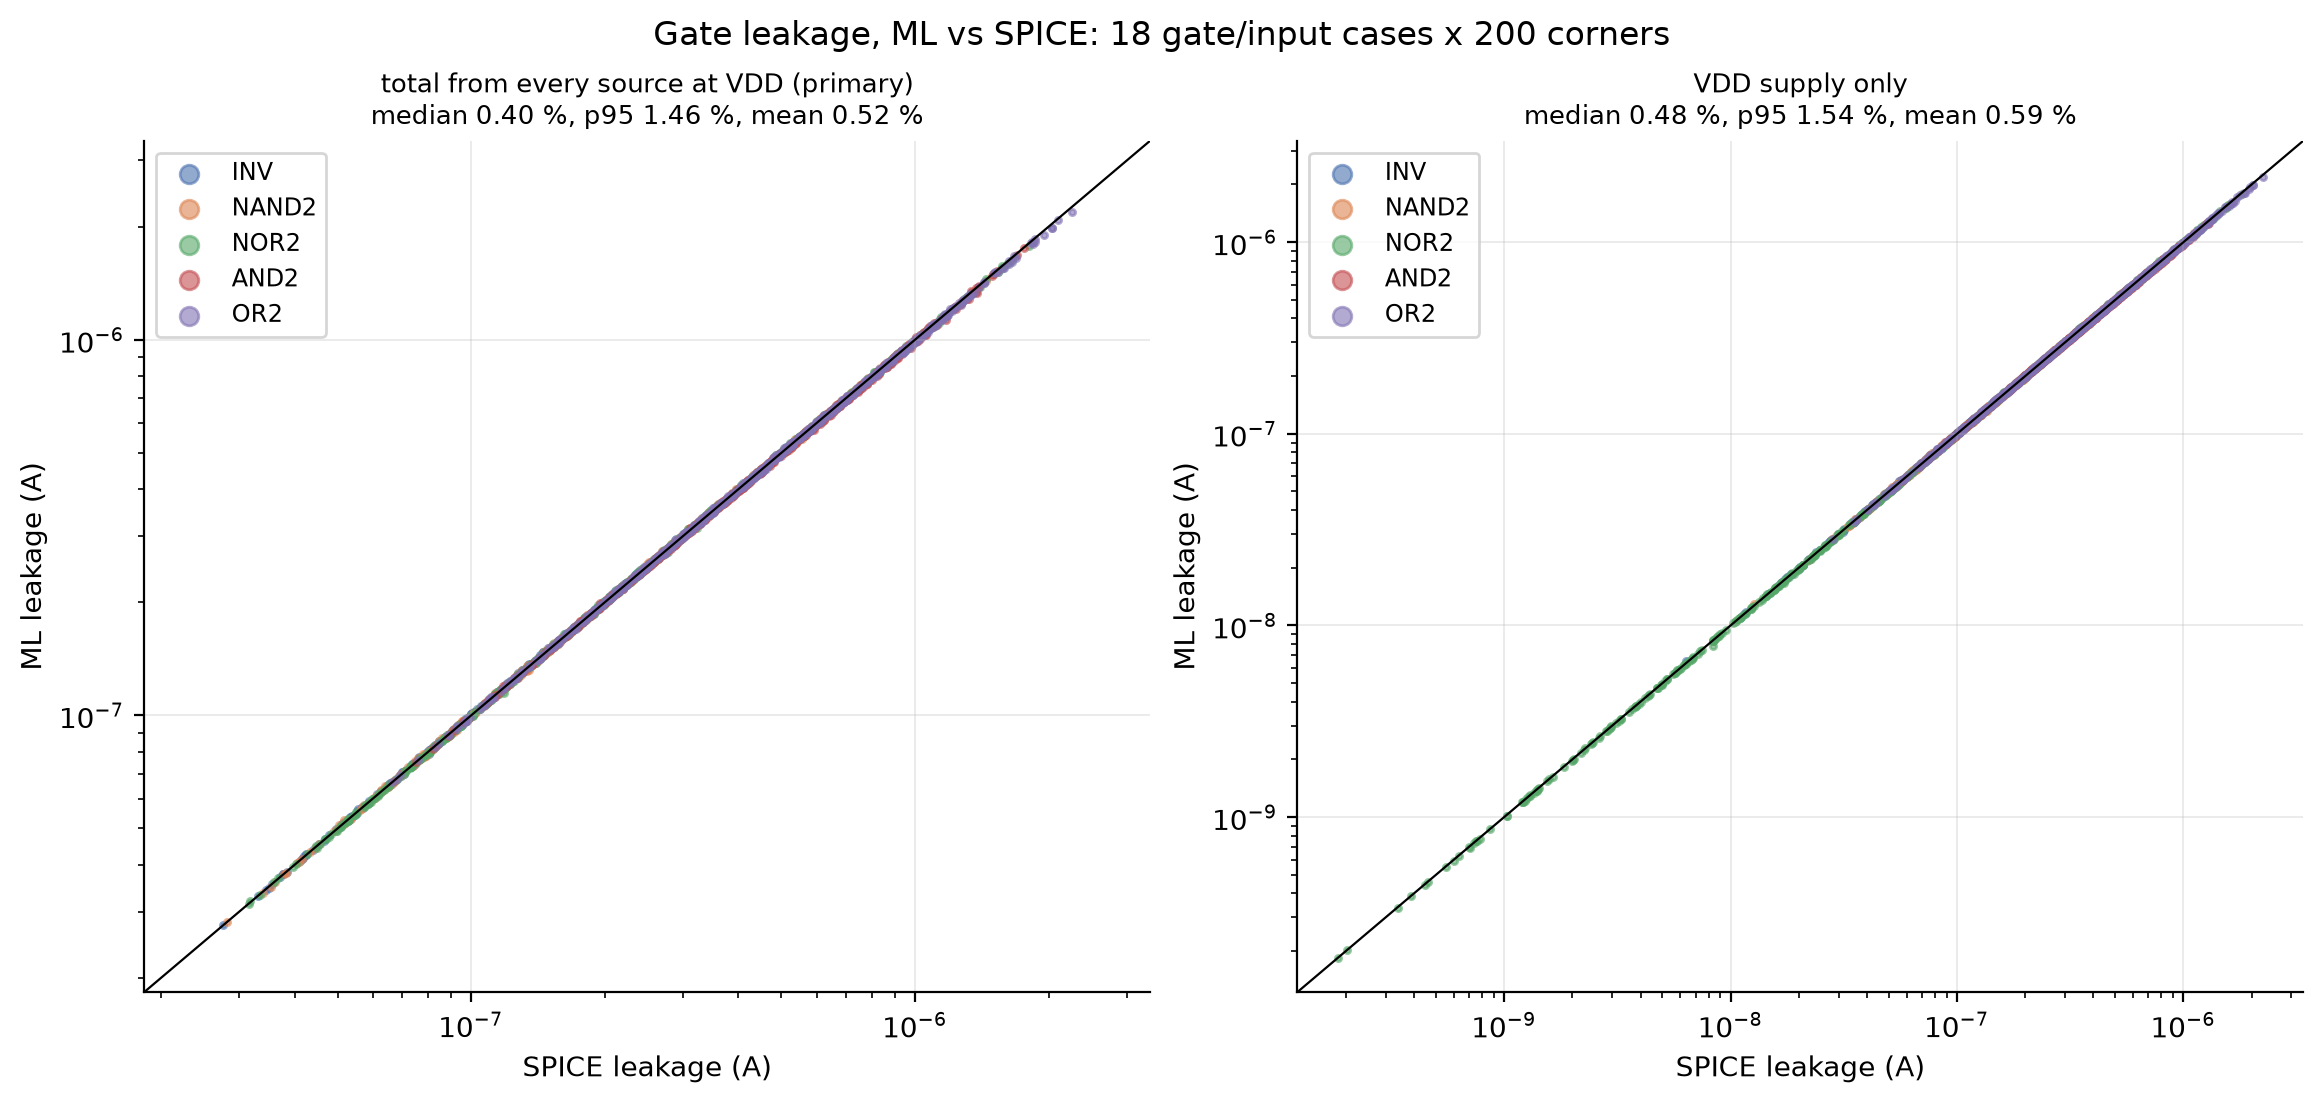
\includegraphics[width=0.85\linewidth]{gates_v3/gate_parity.png}
\caption{Gate parity plot (v3): ML against SPICE leakage for all 3,600 operating points on log axes; total leakage (left) and supply-only leakage (right).}
\label{fig:gparity}
\end{figure}

\noindent\textbf{Most and least accurate cases.} The most accurate cases are INV at A = 1 (median error 0.22\,\%, p95 0.73\,\%), NAND2 at AB = 11 (0.24\,\%, 0.88\,\%) and OR2 at AB = 11 (0.26\,\%, 0.97\,\%). The least accurate are AND2 at AB = 01 and 10 and OR2 at AB = 00 (median 0.78--0.88\,\%, p95 up to 2.26\,\%), the cases with the largest composition floor (0.62--0.67\,\%): their error comes mainly from the inner inverter's gate offset, not from the models. Among single-stage gates, NAND2 at 00 and INV at 0 (0.52\,\% and 0.50\,\%) are least accurate, as gate tunnelling through ON PMOS devices dominates their leakage. The supply-only ranking is the same.

% ==========================================
% SECTION 5: TEST-CIRCUIT RESULTS
% ==========================================
\newpage
\addtocontents{toc}{\protect\thispagestyle{tocpage}}
\section{Test-Circuit Results}
\label{sec:cla}

\keepspace{14\baselineskip}
\subsection{Test Circuit and Method}
\noindent The 3-bit carry-lookahead adder adds $a_2a_1a_0$, $b_2b_1b_0$ and carry-in $c_0$, forming every carry directly from the generate and propagate signals $g_i = a_i b_i$ and $p_i = a_i \oplus b_i$ (for example $c_2 = g_1 + p_1 g_0 + p_1 p_0 c_0$), with sums $s_i = p_i \oplus c_i$. It uses only the gate library: each XOR is four NAND2, giving 39 cells (24 NAND2, 9 AND2, 6 OR2) and 186 transistors. The full transistor-level netlist was simulated in SPICE at all 128 input combinations and the same 200 corners (25,600 operating points); every output equals $A + B + c_0$.

\medskip
\noindent The ML estimate is hierarchical: a logic simulation gives every cell's input bits, and each cell's leakage comes from its gate model at the same corner, with inputs assumed at the rails and no loading between cells. The total leakage is the sum of the cells' total leakages. For the supply-only leakage, only the gate current drawn from primary inputs at logic 1 is subtracted, because a cell input driven by an internal net draws its current from $V_{DD}$ through the driving cell:
\begin{equation}
    I^{\text{CLA}}_{\text{total}} = \sum_{c} I^{c}_{\text{total}}, \qquad
    I^{\text{CLA}}_{\text{supply}} = I^{\text{CLA}}_{\text{total}} - \sum_{c} \sum_{p \in \text{PI}_1(c)} I^{c}_{p}.
    \label{eq:cla}
\end{equation}

\keepspace{287pt}
\subsection{Results}
\noindent Table~\ref{tab:clares} gives the test-circuit metrics and Figure~\ref{fig:claparity} the parity plot. The composition floor sums the exact gate SPICE leakages, and the naive sum adds the cells' supply-only leakages instead of using Eq.~\eqref{eq:cla}.

\begin{table}[H]
\centering
\scriptsize
\begin{tabularx}{\linewidth}{|>{\raggedright\arraybackslash}p{1.1cm}|>{\raggedright\arraybackslash}p{1.7cm}|C|C|C|C|C|C|C|}
\hline
\textbf{Leakage} & \textbf{Estimate} & \textbf{SPICE median ($\mu$A)} & \textbf{ML median ($\mu$A)} & \textbf{Bias (\%)} & \textbf{Median err. (\%)} & \textbf{p95 err. (\%)} & \textbf{Mean err. (\%)} & \textbf{Mean accuracy (\%)} \\
\hline
\multirow{4}{1.1cm}{Total} & ML v1 & 14.08 & 13.99 & $-1.19$ & 0.97 & 4.36 & 1.41 & 98.59 \\
\cline{2-9}
 & ML v2 & 14.08 & 13.99 & $-0.86$ & \textbf{0.73} & 2.81 & 1.01 & 98.99 \\
\cline{2-9}
 & ML v3 & 14.08 & 14.03 & $-0.86$ & 0.82 & \textbf{2.46} & \textbf{0.96} & \textbf{99.04} \\
\cline{2-9}
 & Composition floor & 14.08 & 14.05 & $-0.47$ & 0.44 & 1.70 & 0.59 & 99.41 \\
\hline
\multirow{5}{1.1cm}{Supply only} & ML v1 & 13.08 & 12.99 & $-1.24$ & 1.02 & 4.48 & 1.47 & 98.53 \\
\cline{2-9}
 & ML v2 & 13.08 & 12.99 & $-0.92$ & \textbf{0.79} & 2.91 & 1.06 & 98.94 \\
\cline{2-9}
 & ML v3 & 13.08 & 13.01 & $-0.90$ & 0.87 & \textbf{2.55} & \textbf{1.01} & \textbf{98.99} \\
\cline{2-9}
 & Composition floor & 13.08 & 13.05 & $-0.50$ & 0.47 & 1.77 & 0.63 & 99.37 \\
\cline{2-9}
 & Naive sum (v3) & 13.08 & 10.66 & $-17.29$ & 14.92 & 37.10 & 17.29 & 82.71 \\
\hline
\end{tabularx}
\caption{Test-circuit results over 128 input combinations and 200 corners.}
\label{tab:clares}
\end{table}

\begin{figure}[H]
\centering
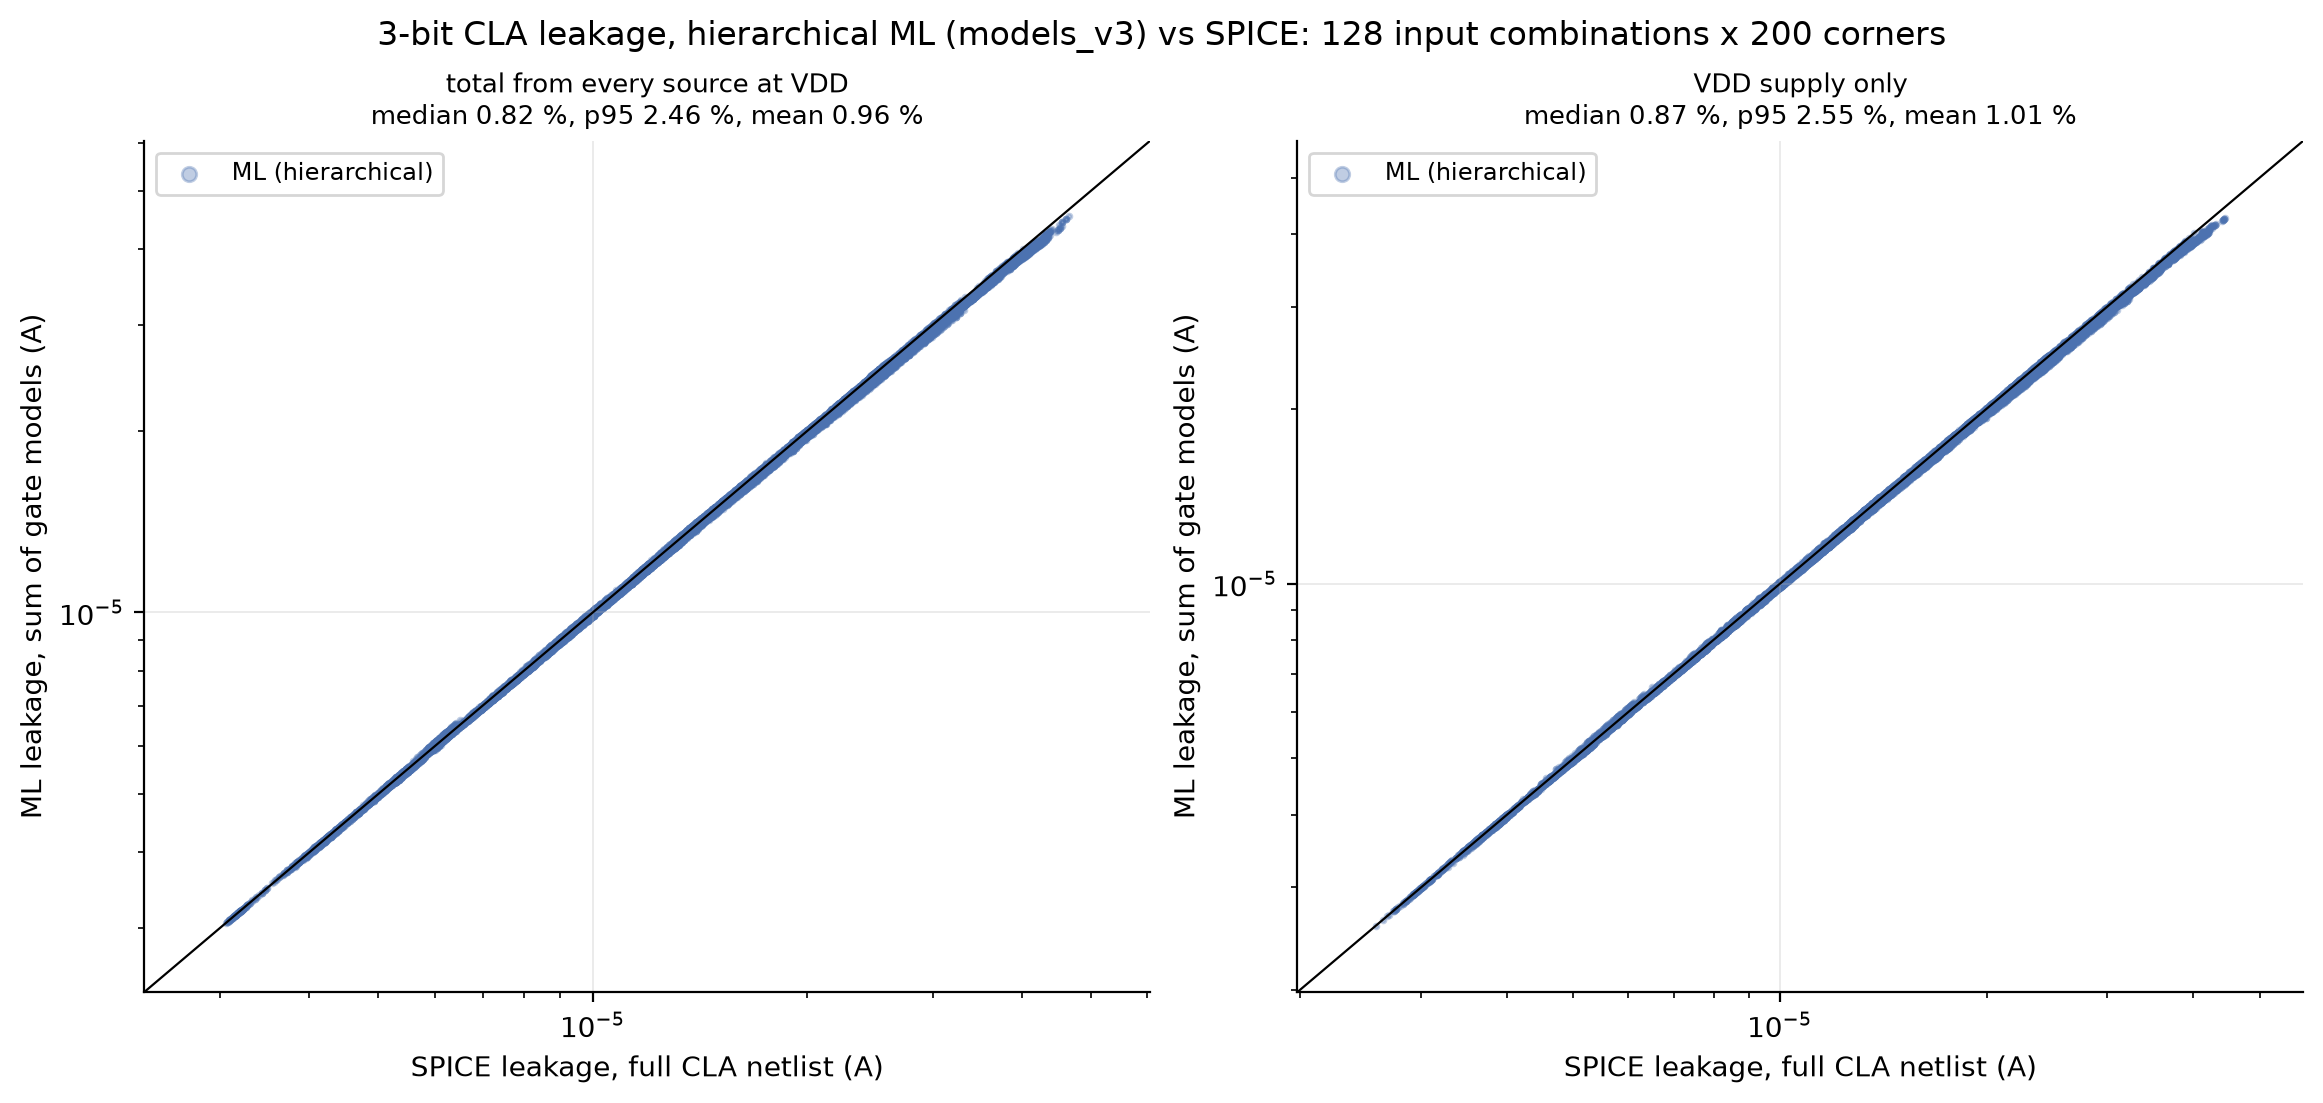
\includegraphics[width=\linewidth]{test_circuit_v3/cla_parity.png}
\caption{Test-circuit parity plot (v3): ML against SPICE leakage for all 25,600 operating points on log axes.}
\label{fig:claparity}
\end{figure}

\noindent\textbf{Comparison with the gates.} With v3 the adder reaches a mean accuracy of 99.04\,\% (total) and 98.99\,\% (supply-only), against 99.48\,\% and 99.41\,\% for the gates. The difference comes from the composition itself: about 0.6 percentage points of mean error remain even with exact gate SPICE values (the composition floor), while the model part alone, ML against the summed gate SPICE leakages, has a mean error of only 0.46\,\%, similar to the gate level. The slightly lower median of v2 arises because part of its model error cancels the negative composition bias; v3 has the lower 95th-percentile and mean errors.

% ==========================================
% SECTION 6: ERROR ANALYSIS
% ==========================================
\newpage
\addtocontents{toc}{\protect\thispagestyle{tocpage}}
\section{Error Analysis}
\label{sec:errors}

\keepspace{14\baselineskip}
\subsection{Transistor Level}
\noindent The largest relative errors of the transistor models occur in three places. The first is near the sign change of $I_d$ and $I_s$ in the OFF cases, where the current is a small difference of large channel and gate parts; each part is predicted accurately, but a small error in either becomes a large relative error. The second is the OFF-state body currents, which change sign near $10^{-17}$\,A. Both carry negligible leakage. The third is operating points with terminals near the rails, which uniform sampling rarely visits but every transistor in a gate occupies; this was the dominant gate-level error source in v1 and v2, and v3 removed it (Table~\ref{tab:v123}).

\keepspace{263pt}
\subsection{Gate Level}
\noindent Table~\ref{tab:corner} shows how the error depends on the corner conditions. In v1 the gate error grows at high temperature, high $V_{DD}$ and high PMOS threshold voltage; the largest v1 error (25.7\,\%, NAND2 at 00) lies in the stacked pull-down, where the upper OFF transistor's source is lifted to $0.1\,V_{DD}$, a region sparsely covered by uniform data. In v3 every correlation is at most 0.13 in magnitude, so the gate error no longer depends on the operating conditions.

\begin{table}[H]
\centering
\small
\begin{tabularx}{\linewidth}{|>{\raggedright\arraybackslash}p{1.6cm}|c|C|C|C|C|C|C|}
\hline
\textbf{Level} & \textbf{Version} & $V_{DD}$ & \textbf{Temp.} & \texttt{vth0} (N) & \texttt{toxe} (N) & \texttt{vth0} (P) & \texttt{toxe} (P) \\
\hline
\multirow{2}{*}{Gates} & v1 & $+0.13$ & $+0.27$ & $-0.04$ & $+0.13$ & $+0.14$ & $+0.12$ \\
\cline{2-8}
 & v3 & $-0.03$ & $+0.13$ & $-0.01$ & $-0.01$ & $+0.03$ & $-0.08$ \\
\hline
\multirow{2}{*}{CLA} & v1 & $+0.15$ & $+0.63$ & $-0.14$ & $+0.14$ & $+0.20$ & $+0.15$ \\
\cline{2-8}
 & v3 & $-0.09$ & $+0.73$ & $-0.18$ & $+0.05$ & $+0.23$ & $+0.05$ \\
\hline
\end{tabularx}
\caption{Spearman rank correlation of the absolute error (total leakage) with corner variables.}
\label{tab:corner}
\end{table}

\noindent Table~\ref{tab:worst} splits the five largest v3 gate errors into the composition floor and the model part. Four of the five are AND2 or OR2 at high temperature, where most of the error is the inner inverter's gate offset; the remaining one (NOR2 at 11) is a 4\,\% underestimate of the ON-state NMOS gate current at 97\,$^{\circ}$C.

\begin{table}[H]
\centering
\small
\begin{tabularx}{\linewidth}{|>{\raggedright\arraybackslash}p{1.6cm}|c|>{\raggedright\arraybackslash}p{3.4cm}|C|C|C|}
\hline
\textbf{Gate, AB} & \textbf{Corner} & \textbf{Conditions} & \textbf{ML error} & \textbf{Composition floor} & \textbf{Model part} \\
\hline
AND2, 10 & 123 & 110\,$^{\circ}$C, 1.044\,V, NMOS \texttt{vth0} $-9.1\,\%$ & $-3.62$ & $-2.19$ & $-1.43$ \\
\hline
NOR2, 11 & 145 & 97\,$^{\circ}$C, 1.090\,V, NMOS \texttt{vth0} $-6.5\,\%$ & $-3.13$ & $0.00$ & $-3.13$ \\
\hline
AND2, 10 & 145 & 97\,$^{\circ}$C, 1.090\,V & $-3.09$ & $-1.53$ & $-1.56$ \\
\hline
AND2, 10 & 186 & 121\,$^{\circ}$C, 0.959\,V, NMOS \texttt{vth0} $-9.1\,\%$ & $-3.08$ & $-3.20$ & $+0.12$ \\
\hline
OR2, 00 & 109 & 82\,$^{\circ}$C, 1.075\,V, NMOS \texttt{vth0} $+9.7\,\%$ & $-3.07$ & $-1.61$ & $-1.46$ \\
\hline
\end{tabularx}
\caption{The five largest v3 gate errors (total leakage, \%).}
\label{tab:worst}
\end{table}

\keepspace{293pt}
\subsection{Test-Circuit Level}
\noindent The adder error grows strongly with temperature in every version ($\rho \approx 0.7$, Table~\ref{tab:corner}). Table~\ref{tab:clatemp} shows that this is mainly a composition effect: the composition bias grows from $+0.06\,\%$ to $-1.05\,\%$ from the lowest to the highest temperature third, while the model part grows much less. Internal nets at logic 1 drive cell inputs with slightly degraded levels, which the gate models (inputs exactly at the rails) do not see, so the adder leaks more than the sum of its isolated gates; accordingly, the bias correlates with the number of internal nets at 1 ($\rho = -0.90$ for the composition floor). Errors that are common to many cells add up over the 39 cells, while isolated cell errors are diluted.

\begin{table}[H]
\centering
\small
\begin{tabularx}{\linewidth}{|>{\raggedright\arraybackslash}p{2.6cm}|c|C|C|C|C|}
\hline
\textbf{Temperature third} & \textbf{Range ($^{\circ}$C)} & \textbf{Median err.} & \textbf{Bias} & \textbf{Composition bias} & \textbf{Model part, median} \\
\hline
Low & $-39$ -- 20 & 0.39 & $-0.15$ & $+0.06$ & 0.29 \\
\hline
Middle & 21 -- 74 & 0.80 & $-0.78$ & $-0.44$ & 0.38 \\
\hline
High & 75 -- 124 & 1.53 & $-1.65$ & $-1.05$ & 0.58 \\
\hline
\end{tabularx}
\caption{Test-circuit error (v3, total leakage, \%) by temperature.}
\label{tab:clatemp}
\end{table}

% ==========================================
% SECTION 7: LIMITATIONS AND IMPROVEMENTS
% ==========================================
\newpage
\addtocontents{toc}{\protect\thispagestyle{tocpage}}
\section{Limitations and Improvements}
\label{sec:limits}

\keepspace{14\baselineskip}
\subsection{Limitations}
\begin{itemize}[leftmargin=*]
    \item \textbf{Gate voltages only at the rails.} The transistor models represent gates exactly at 0 or $V_{DD}$, so gates driven by internal nodes a few millivolts from a rail (the inverters of AND2 and OR2, and every cell inside the adder) are not represented exactly. This is the main remaining error at gate level.
    \item \textbf{No loading between cells.} The hierarchical estimate sums isolated gate leakages; loading and degraded logic levels between cells cost about 0.6 percentage points of mean accuracy at circuit level and grow with temperature.
    \item \textbf{Relative error of near-zero currents.} Currents that are small differences of large parts (near a sign change, or the body current) have large relative errors, although they carry almost no leakage.
\end{itemize}

\keepspace{14\baselineskip}
\subsection{Improvements}
\begin{itemize}[leftmargin=*]
    \item \textbf{Gate voltage as a model input.} Training with the gate voltage varied slightly around each rail would remove the inner-gate offset error of AND2 and OR2 and much of the adder's composition error.
    \item \textbf{Loading-aware composition.} Propagating the predicted logic level of each internal net from cell to cell, instead of assuming exact rails, would address the composition bias at circuit level.
    \item \textbf{Bias correction.} Because errors common to many cells accumulate in a circuit, calibrating out the residual mean bias of the gate models would directly improve circuit-level accuracy.
    \item \textbf{Sampling around operating points.} Rail-focused sampling was the most effective improvement; sampling designed around other critical operating points, such as stack nodes between two OFF transistors, would extend it.
\end{itemize}

% ==========================================
% SECTION 8: CONTRIBUTIONS
% ==========================================
\keepspace{565pt}
\addtocontents{toc}{\protect\thispagestyle{tocpage}}
\section{Contributions}
\label{sec:contrib}

\noindent The work was divided so that each member owned one stage of the pipeline and one further component of comparable size. Each member wrote the report sections on their own work, and all members reviewed the complete results.

\begin{table}[H]
\centering
\small
\begin{tabularx}{\linewidth}{|>{\raggedright\arraybackslash}p{3.6cm}|L|}
\hline
\textbf{Member} & \textbf{Contributions} \\
\hline
Vishnubhotla Nitin Sri Siva Kalyan (2024112012) &
\vspace{-0.9em}
\begin{itemize}[leftmargin=*, nosep, topsep=0pt]
    \item Transistor data generation: PVT and bias sampling, single-transistor netlists with source/drain geometry, and the batch SPICE simulation of the four 10,000-sample datasets.
    \item Data check: Kirchhoff check of all samples and the three trend plots with controlled SPICE sweeps.
    \item Test circuit: design of the 3-bit carry-lookahead adder from the gate library and its full transistor-level SPICE reference over 128 inputs and 200 corners.
\end{itemize}
\vspace{-0.9em} \\
\hline
Anay Rungta (2024102050) &
\vspace{-0.9em}
\begin{itemize}[leftmargin=*, nosep, topsep=0pt]
    \item Proposed and generated the rail-focused samples, which target the operating region of transistors inside gates.
    \item v3 models: physics-based input features, training with the rail-focused data, and evaluation on the rail-focused test set.
    \item Error analysis: dependence of the errors on corner conditions, and the tracing of the largest gate errors to their composition and model parts.
\end{itemize}
\vspace{-0.9em} \\
\hline
Alapati Sai Pavan Adit (2024102064) &
\vspace{-0.9em}
\begin{itemize}[leftmargin=*, nosep, topsep=0pt]
    \item Learning targets and preprocessing: the Kirchhoff-consistent target split and input features of the transistor models.
    \item Model comparison: the four model types, their hyperparameter grids, selection on the validation set and the learning curve.
    \item v2 models: training on the additional uniform data and averaging of independently trained networks.
\end{itemize}
\vspace{-0.9em} \\
\hline
Vidvathama R (2024122002) &
\vspace{-0.9em}
\begin{itemize}[leftmargin=*, nosep, topsep=0pt]
    \item Gate library and SPICE reference: transistor-level netlists of the five gates and their simulation at 18 input cases and 200 corners.
    \item Gate-level ML estimate: composition of gate leakage from the transistor models by Kirchhoff's law, for both leakage definitions.
    \item Hierarchical test-circuit estimate: cell-level composition of the adder leakage and the supply-only correction.
\end{itemize}
\vspace{-0.9em} \\
\hline
\end{tabularx}
\caption{Contributions of the team members.}
\label{tab:contrib}
\end{table}

\end{document}
